%\documentclass[a4paper]{article}
%\usepackage{graphicx,placeins}
%\usepackage{epsfig}
%\usepackage{comment}
%\usepackage{amsmath,amsthm}
%\usepackage{xspace}
%\usepackage[colorlinks=true,citecolor=blue]{hyperref}
%\usepackage[acronym,nonumberlist,nogroupskip]{glossaries}
%\usepackage{showlabels}
%\usepackage{titlesec}
%\setcounter{secnumdepth}{4}
%\titleformat{\paragraph}
%{\normalfont\normalsize\bfseries}{\theparagraph}{1em}{}
%\titlespacing*{\paragraph}
%{0pt}{3.25ex plus 1ex minus .2ex}{1.5ex plus .2ex}
%
%\newcommand{\etal}{{\it et~al.}\ }
%\newcommand{\ie}{{\it i.e.}\ }
%\newcommand{\eg}{{\it e.g.}\ }
%\newcommand{\Ito}{It\^{o} }
%\newcommand{\tsing}{t_{\text{singular}}}
%\newcommand{\gest}{g_{\text{est}}}
%\newcommand{\eq}{\hspace{-.15cm}=\hspace{-.15cm}}
%
%\newcommand{\ave}[1]{\left\langle#1 \right\rangle}
%\newcommand{\dist}{\,{\buildrel d \over =}\,}
%\newcommand{\mut}{\tilde{\mu}}
%\newcommand{\sigmat}{\tilde{\sigma}}
%\newcommand{\var}{\text{var}}
%\newcommand{\stdev}{\text{stdev}}
%
%\newcommand{\rex}{r_{\ave{}}}
%\newcommand{\rt}{r_{t}}
%
%\newcommand{\gt}{g_{t}}
%\newcommand{\gex}{g_{\ave{}}}
%
%
%\newcommand{\elabel}[1]{\label{eq:#1}}
%\newcommand{\eref}[1]{(Eq.~\ref{eq:#1})}
%\newcommand{\Eref}[1]{Equation~(\ref{eq:#1})}
%
%\newcommand{\ceref}[2]{(\ref{eq:#1}#2)}
%
%\newcommand{\tlabel}[1]{\label{tab:#1}}
%\newcommand{\tref}[1]{(Table~\ref{tab:#1})}
%
%\newcommand{\flabel}[1]{\label{fig:#1}}
%\newcommand{\fref}[1]{Fig.~\ref{fig:#1}}
%\newcommand{\Fref}[1]{Figure ~\ref{fig:#1}}
%
%\newcommand{\seclabel}[1]{\label{section:#1}}
%\newcommand{\secref}[1]{Sec.~\ref{section:#1}}
%\newcommand{\Secref}[1]{Section~\ref{section:#1}}
%
%\newcommand{\OP}[1]{{\bf @@@OP: #1 @@@}}
%\renewcommand{\AA}[1]{{\bf ===AA: #1 ===}}
%
%\newcommand{\be}{\begin{equation}}
%\newcommand{\ee}{\end{equation}}
%\newcommand{\bea}{\begin{eqnarray}}
%\newcommand{\eea}{\end{eqnarray}}
%\newcommand{\bc}{\begin{center}}
%\newcommand{\ec}{\end{center}}
%\newcommand{\prob}[1]{\mathcal{P}\left(#1\right)}
%\newcommand{\D}{\Delta}
%\newcommand{\PDF}{\mathcal{P}}
%\newcommand{\nn}{\nonumber}
%
%\newcommand{\definition}[1]{\vspace{.2cm} {\bf \underline{Definition} #1} \vspace{.2cm}}

\newpage

\section{Populations}
{\it 
The previous chapter developed a model of individual behaviour based on an
assumed dynamic imposed on wealth. If we know the stochastic process that describes
individual wealth, then we also know what happens at population level -- each individual
is represented by a realisation of the process, and we can compute 
the dynamics of wealth distributions. We answer questions about inequality and poverty in
our model economy. It turns out that our decision criterion generates interesting emergent
behaviour -- cooperation, the sharing and pooling of resources, is often time-average 
growth optimal. This provides answers to the puzzles of why people cooperate, why there 
is an insurance market, and why we see socio-economic structure from the formation of 
firms to nation states with taxation and redistribution systems.}
\newpage

\subsection{Every man for himself}
\seclabel{Every_man}

We have seen that risk aversion constitutes optimal behaviour under the assumption 
of multiplicative wealth growth and over time scales that are long enough for systematic 
trends to be significant. In this chapter we will continue to explore our null model, 
GBM. By ``explore'' we mean that we will let the model generate its world -- if 
individual wealth was to follow GBM, what kind of features of an economy would emerge? 
We will see that cooperation and the formation of social structure also constitute 
optimal behaviour.

GBM is more than a random variable, it's a stochastic process, \ie a set of trajectories 
$x(t)$ or  a family of random variables parameterized by $t$, depending on how we 
prefer to look at it.  Both perspectives are informative in the context of economic modelling
-- from the set of trajectories we can judge what is likely to happen to an individual, 
\eg by following an individual trajectory for a long time, and the PDF of the random 
variable $x(t^*)$ at some fixed value of $t^*$ is the wealth distributed in our model. 

We use the term wealth distribution to refer to the density function 
$\PDF_x(x)$ (not to the process of distributing wealth among people). This can be 
interpreted as follows: if I select a random individual (each individual with uniform probability 
$\frac{1}{N}$), the probability of the selected individual 
having wealth greater than $x$ is given by the CDF $F_x(x)=\int_x^\infty ds \PDF_x(s)$.
In a large population of $N$ individuals, $\D x \PDF_x(x)N$ is the approximate 
number of individuals who have wealth near $x$. 
Thus, a broad wealth distribution with heavy tails indicates greater wealth inequality. 

\underline{Examples:}
\begin{itemize}
\item Under perfect equality everyone would have the same, meaning that the wealth
distribution would be a Dirac delta function centered at the mean of $x$, that is
\be
\PDF_x(x)=\delta(x-\ave{x}_N);
\ee
\item
Maximum inequality would mean that one individual owns everything
and everyone else owns nothing, that is
\be 
\PDF_x(x)=\frac{N-1}{N}\delta(x-0)+\frac{1}{N}\delta(x-N\ave{x}_N).
\ee
\end{itemize}

\subsubsection{Log-normal wealth distribution}
\seclabel{Log-normal_wealth}
GBM is log-normally distributed. If each individual's wealth follows GBM,
\be
dx=x(\mu dt + \sigma dW),
\elabel{GBM}
\ee
with solution 
\be
x(t) = x_0 \exp\left[\left(\mu-\frac{\sigma^2}{2}\right)t + \sigma W(t)\right],
\ee
then we will observe a log-normal wealth distribution at each moment in time:
\be
\ln x(t) \sim \mathcal{N}\left(\ln x_0 + \left(\mu - \frac{\sigma^2}{2}\right)t, \sigma^2 t\right).
\elabel{lognormal}
\ee


We notice that the variance of $\ln x$ increases linearly in time -- 
we will develop an understanding of this fact shortly. As we will see 
(though we cannot conclude this yet), it indicates that any meaningful 
measure of inequality will grow over time in our simple model. 
To see what kind of a wealth distribution \eref{lognormal} is, it is worth 
spelling out the lognormal PDF
\be
\PDF(x)=\frac{1}{x\sqrt{2\pi \sigma^2t}}\exp\left(-\frac{[\ln(x)-(\mu-\frac{\sigma^2}{2})t]^2}{2\sigma^2 t} \right).
\elabel{PDFx}
\ee

INSERT PROPERTIES OF GBM DISTRIBUTION HERE (note that lognormal is an insufficient description of the distribution of a GBM - the time-dependence of the random variable must be included)

It is a well-established empirical observation \cite{Newman2005} that the upper tails of 
real wealth distributions tend to look more like a power law than a log-normal. Our trivial model does not
strictly reproduce this feature, but it is instructive to compare the lognormal distribution
to a power-law distribution. A power law PDF has the aymptotic form 
\be
\PDF_x(x)= x^{-\alpha},
\elabel{power_law}
\ee
for large arguments $x$. This implies that the logarithm of the PDF is proportional 
to the logarithm of its argument, $\ln \PDF_x(x) = -\alpha \ln x$. Plotting
one against the other will yield a straight line, the slope being the exponent $-\alpha$. 

Determining whether an empirical observation is consistent with such behaviour 
is difficult because the behaviour is to be observed in the tail (large $x$) where data are
by definition sparse. A quick-and dirty way of checking for possible power-law 
behavior is to plot an empirical PDF against its argument on log-log scales, 
look for a straight line, and measure the slope. However, plotting any distribution on any 
type of scales results in some line. It may not be a straight line but it will have some slope 
everywhere. For a known distribution (power law or not) we can interpret this slope 
as a local apparent power-law exponent. 

What is the local apparent power-law exponent of a log-normal wealth distribution near the 
expectation value $\ave{x}$, \ie in the upper tail where approximate power law behavior
has been observed empirically? The logarithm of \eref{PDFx} is
\bea
\ln \PDF(x)&=&-\ln x\sqrt{2\pi \sigma^2t} -\frac{([\ln(x)-(\mu-\frac{\sigma^2}{2})t]^2}{2\sigma^2 t}\\
&=&-\ln x -\frac{\ln (2\pi \sigma^2t)}{2} - \frac{(\ln(x)^2+[(\mu-\frac{\sigma^2}{2})t]^2-2(\mu-\frac{\sigma^2}{2})t \ln x}{2\sigma^2 t}
\eea
Collecting terms in powers of $\ln x$ we find
\be
\ln \PDF(x)=[\ln x]^2 \times\frac{-1}{2\sigma^2 t}  + \ln x \times \left(-\frac{3}{2}+\frac{\mu}{\sigma^2} \right) -\frac{\ln(2 \pi\sigma^2 t)}{2}-\frac{[(\mu-\frac{\sigma^2}{2})t]^2}{2\sigma^2 t}
\ee
with local slope, \ie apparent exponent,
\be
\frac{d\ln \PDF(x)}{d \ln x}=-\frac{\ln x}{\sigma^2 t}  - \frac{3}{2}+\frac{\mu}{\sigma^2}.
\ee
If the first term is small compared to the others, this distribution will look like a power law when
plotted on double-logarithmic scales. We don't believe that the empirically observed power laws
are merely a manifestation of this mathematical feature. Important real-world  mechanisms 
that broaden real wealth distributions, \ie concentrate wealth, are missing from the 
null model. However, it is interesting that the trivial model of GBM chimes with so many qualitative 
features of empirical observations. 

\subsubsection{Inequality measure from two growth rates}
\seclabel{Inequality_measure}
In the case of GBM we have just seen how to 
compute the exact full wealth distribution $\PDF$. This is intersting, but
we often only want summary measures of the distribution. A distributional property of particular 
interest to economists is inequality. How much inequality is there in a distribution like \eref{lognormal}, 
and in what sense does this quantity increase in time under GBM as we have pointed out?
Clearly, we should quantify ``inequality''. In this section we develop a natural way of measuring it, 
which makes use of the two growth rates we identified for the non-ergodic process. We will see 
that a particular inequality measure, known to economists as
Theil's second index of inequality \cite{Theil1967}, is the difference
between typical wealth (that grows at the time-average growth rate) and average wealth 
(that grows at the ensemble-average growth rate) in our model. Thus, the difference between
the time average and ensemble average, the essence of ergodicity breaking, 
fundamentally drives  the dynamics of inequality.

The two limits of inequality are easily identified: minimum inequality means that everyone 
has the same wealth, and maximum inequality means that one individual has all the 
wealth and everyone else has nothing (this assumes that wealth cannot become 
negative). Quantifying inequality in any other distribution is reminiscent of the gamble 
problem. Recall that for gambles we wanted make statements of the type ``this gamble 
has more desirability than that gamble''. We did this by collapsing a distribution to a 
scalar. Depending on the question that was being asked 
the appropriate way of collapsing the distribution and the resulting scalar can be different 
(the scalar relevant to an insurance company may not be relevant to an individual). 
In the case of inequality we also have a distribution -- the wealth distribution -- and we 
want to make statements of the type ``this distribution has more inequality than that 
distribution''. Again, this is done by collapsing the distribution to a scalar, and again 
many different choices of collapse and resulting scalar are possible. The Gini 
coefficient is a particularly well-known scalar of this type, the 80/20 ration is another, 
and many other measures exist.

In this context the expectation value is an important quantity. 
%Allowing initial wealth, 
%$x_0$, to be a random variable, the mean of the wealth distribution \eref{lognormal} is
%\be
%\ave{x(t)}=\ave{x_0}e^{\mu t}.
%\ee
For instance, if everyone has the same wealth, everyone will own the average $\forall i, x_i=\ave{x}_N$,
which converges to the expectation value for large $N$. Also, whatever the distribution 
of wealth, the total wealth is $N\ave{x}_N$ which converges to $N\ave{x}$. The growth 
rate of the expectation value, $\gex$, thus tells us how fast the average wealth and the 
total population wealth grow with probability one in a large ensemble. The time-average 
growth rate, $\gt$, tells us how fast an individual's wealth grows with probability one in 
the long run. If the typical individual's wealth grows at a lower rate than the 
expectation value of wealth then there must be a-typical individuals with very large 
wealth that account for the difference. This suggests the following measure of 
inequality.

\definition{
inequality $J(t)$, is the quantity that grows in time at the rate of the 
difference between expectation-value and time-average growth rates,
%The inequality present in the distribution does not depend on absolute 
%wealth levels, which is one of four criteria that together define so-called ``relative inequality 
%measures'' \cite[p.~139]{Sen1997}. It is convenient to divide everyone's wealth by the 
%common factor $\ave{x}$ and focus on the rescaled wealth,
%\be
%y \equiv \frac{x}{\ave{x}} = \frac{xe^{-\mu t}}{\ave{x_0}},
%\elabel{ydef}
%\ee
%This is done purely for mathematical convenience and does not affect any reasonable measure of inequality.
%The SDE for $y$ is obtained by applying \Ito's version of the chain rule for SDEs: 
%\bea
%dy &=& \frac{\partial y}{\partial t}\,dt + \frac{\partial y}{\partial x}\,dx + \frac{1}{2} \frac{\partial^2 y}{\partial x^2} \,dx^2 \\
%&=& -\mu y\,dt + \frac{y}{x}\,dx \elabel{ysde} \\
%&=& y\sigma\,dW.
%\eea
%The rescaled wealth remains distributed as a continually-broadening lognormal but it no longer depends on the drift,
%\be
%\ln y(t) \sim \mathcal{N}\left(-\frac{\sigma^2 t}{2}, \sigma^2 t\right).
%\elabel{y_lognorm}
%\ee
%It has constant unit mean, which is trivially shown by noting that
%\be
%\ave{y} = \ave{\frac{x}{\ave{x}}} = 1.
%\elabel{ymean}
%\ee
\be
\frac{dJ}{dt}=\gex-\gt.
\elabel{dJ}
\ee
\Eref{dJ} defines the dynamic of inequality, and inequality itself is found by 
integrating over time
\be
J(t)=\int_0^t ds [\gex(s)-\gt(s)].
\elabel{J}
\ee
}

This definition may be used for dynamics other than
GBM. Whatever the wealth dynamic, typical minus average growth rates are informative of the
dynamic of inequality. Within the GBM framework we can write down the two growth rates 
explicitly and find 
\be
\frac{dJ}{dt}=\frac{d \ln \ave{x}}{dt}-\frac{d \ave{\ln x}}{dt}.
\elabel{J_dyn}
\ee
Integrating over time
\be
J(t)=\ln \ave{x}-\ave{\ln x},
\ee
which is known as the mean logarithmic deviation (MLD) or Theil's second index of inequality \cite{Theil1967}. 
This is rather remarkable. Our general inequality measure, \eref{J}, evaluated 
for the specific case of GBM, turns out to be a well-known measure of inequality that 
economists identified independently, without considering non-ergodicity and ensemble 
average and time average growth rates. Merely by insisting of measuring inequality well,
Theil implicitly used the GBM model!

The expectation value $\ave{\ln x}=\ln x_0 + \left(\mu - \frac{\sigma^2}{2}\right)t$ is
given by \eref{lognormal}. It differs from the logarithm of the expectation value, 
$\ave{\ln x}\neq \ln\ave{x}$, which we now compute. In order to do this we introduce 
a useful trick that will come in handy again in \secref{Wealth_tax} (the general 
procedure is described in \cite[Chapter 4.2]{KloedenPlaten1992}): to compute
moments, $\ave{x^n}$, of stochastic differential equations for $x$,  like 
\eref{GBM}, we find solvable ordinary differential equations for the moments. 
For the first moment we do this simply by taking expectations of both sides of \eref{GBM}.
The noise term disappears, and we turn the SDE for $x$ into an ODE for $\ave{x}$
\bea
\ave{dx}&=&\ave{x(\mu dt + \sigma dW)}\\
d\ave{x}&=&\ave{x} \mu dt + \sigma \overbrace{\ave{dW}}^{=0}\\
&=&\ave{x} \mu dt.
\eea
This is a (very simple) first order linear differential equation for 
the first moment (\ie the expectation value) of $x$. Its solution is
\be
\ave{x}=\ave{x_0} \exp(\mu t)
\elabel{exp_x}
\ee
so that $\ln\ave{x}=\ln \ave{x_0} + \mu t$.  Now we can carry out the differentiations
on the RHS of \eref{J_dyn} and find the Theil inequality as a function of time
\be
J(t)=J(0)+\frac{\sigma^2}{2} t.
\ee
Inequality increases indefinitely. This result implies an evolution towards wealth condensation. Wealth condensation 
means that a single individual will own a non-zero fraction of the total wealth in the 
population in the limit of large $N$, see \eg \cite{BouchaudMezard2000}. In the 
present case an arbitrarily large share of total wealth will be owned by an arbitrarily 
small share of the population. 


Over the decades, economists have arrived at many inequality measures, and have drawn 
up a list of conditions that particularly useful measures of inequality satisfy. Such measures
are called ``relative measures'' \cite[Appendix 4]{Sen1997}, and $J$ is one of them. One of the conditions is that inequality measures
should not change when $x$ is divided by the same factor for everyone. Since we are primarily 
interested in inequality in this section it is useful to remove absolute wealth levels from the
analysis and study an object called the rescaled wealth.

\definition{
The rescaled wealth, 
\be
y=\frac{x}{\ave{x}_N},
\elabel{rescaled}
\ee
is the proportion of the population-average wealth owned by an individual.}

This quantity is useful, for instance because its numerical value does not 
depend on the currency used, it is a dimensionless number. 
Thus if my rescaled wealth, $y=1/2$, this means that my wealth is half the 
average wealth, irrespective of whether I measure wealth in Kazakhstani Tenge 
or in Swiss Francs. \Eref{J_dyn}, may be expressed in 
terms of $y$ as $\frac{dJ}{dt}=-\frac{d\ave{\ln y}}{dt}$. 

%One way of seeing this is to calculate the fraction of 
%the population whose wealths are less than the mean. From \eref{y_lognorm} we 
%define a new variable, z, whose distribution is the standard normal:
%\be
%z \equiv \frac{\ln y + \sigma^2t/2}{\sigma t^{1/2}} \sim \mathcal{N}(0,1).
%\ee
%We are interested in the mass of the distribution with $\ln y<0$, which is simply
%\be
%\prob{z<\frac{\sigma t^{1/2}}{2}} = \Phi\left(\frac{\sigma t^{1/2}}{2}\right),
%\ee
%where $\Phi$ is the standard normal cdf. This fraction tends to one as $t\to\infty$.

\subsection{Sums of lognormals and the random energy model}
\seclabel{REM}

\subsubsection{Introduction -- why study GBM?}
The basic phenomenon of self-reproduction occurs from the 
smallest chemical compound capable of building copies of itself to arguably the most complex 
known social system, namely the global economy. Not only is the economy made by humans 
who self-reproduce and whose cells self-reproduce but capitalism itself taps into the power of 
self-reproduction: capital means resources which can be deployed in order to 
generate resources, which can be deployed in order\dots. Realism usually requires models that include noise, to account for the multitude of effects not explicitly modelled. GBM is a simple, intuitive, and analytically tractable model of noisy multiplicative growth. 
A deep understanding of this basic model of self-reproduction is crucial and only in the last few decades have 
we achieved this. 

A quantity, $x$, of self-reproducing resources (such as biomass or capital) follows GBM if it evolves over time, $t$, according to the \Ito stochastic differential equation,
\be
dx=x(\mu dt+\sigma dW_t).
\elabel{GBM}
\ee
$dt$ denotes the infinitesimal time increment and $dW_t$ the infinitesimal increment in a Wiener process, which is a normal variate with $\ave{dW_t}=0$ and $\ave{dW_t dW_s}=\delta(t-s) dt$. $\mu$ and $\sigma$ are constant parameters called the drift and volatility. Put simply, relative changes in resources, $dx/x$, are assumed to be drawn independently from a stationary normal distribution at each time step. \eref{GBM} represents the continuous-time limit of this process. Its solution,
\be
x(t)=x(0)\exp\left[\left(\mu-\frac{\sigma^2}{2}\right) t+\sigma W(t)\right],
\elabel{GBM_sol}
\ee
yields exponential growth at a noisy rate. Hereafter, we shall assume $x(0)=1$ and neglect it, except where retaining it is illustrative. The distribution of $x(t)$ is a time-dependent log-normal,
\be
\ln(x(t)) \sim \mathcal{N}\left( \left(\mu-\frac{\sigma^2}{2}\right)t,\, \sigma^2 t \right),
\ee
whose mean, median, and variance grow (or decay) exponentially in time:
\bea
\ave{x(t)} &=& \exp(\mu t); \elabel{mean_x}\\
\text{median}(x(t)) &=& \exp[(\mu-\sigma^2/2)t]; \elabel{median_x}\\
\text{var}(x(t)) &=& \exp(2\mu t)[\exp(\sigma^2t)-1]. \elabel{var_x}
\eea

GBM is a standard model in finance for self-reproducing quantities such as stock prices. Since relative changes are modelled as normal variates, the central limit theorem means that GBM is an attractor process for a large class of multiplicative dynamics. Any quantity whose relative changes are random variables with finite mean and variance will behave 
like a GBM after a sufficiently long time. We work with GBM because it is standard and general. It exemplifies important qualitative and universal features
of multiplicative growth.

Specifically, we are interested in GBM as a model of economic resources, owned by some entity. We will think of $x$ as measured in currency units, such as dollars.

\subsubsection{Non-ergodicity of GBM}
The non-ergodicity of this growth process
manifests itself in an intriguing way as a difference between the growth of the expectation
value of $x$ and the growth of $x$ over time. Imagine a world where people's wealth 
follows \eref{GBM}. In such a world each person's wealth grows exponentially at rate
\be
g_t=\mu-\sigma^2/2
\elabel{gt}
\ee
with probability 1 if we observe the person's wealth for a long time.
The expectation value of each person's wealth grows exponentially at
\be
g_{\ave{}}=\mu.
\elabel{gave}
\ee
The expectation value, by definition, is the average over an ensemble of $N$ realizations of
$x$ in the limit $N\to\infty$. Important insights follow: the aggregate wealth in our model 
economy does not grow at the same rate as an individual's wealth \cite{AdamouPeters2016} (meaning that GDP may be a flawed reflection of national
economic well-being); inequality grows indefinitely \cite{BouchaudMezard2000,BermanPetersAdamou2017} (even without interactions between individuals); and 
pooling and sharing resources accelerates growth \cite{PetersAdamou2015a,Bouchaud2015}.

\subsubsection{PEAs in GBM -- a sketch\seclabel{sketch}}
The following question often emerges in applications of these results. \Eref{gt} and \eref{gave} are limiting cases ($t \to \infty$ and $N\to\infty$, respectively): what happens when time and population size are finite? In \cite{PetersKlein2013} we studied the ``partial ensemble average'' (PEA) of GBM, details of which are in \secref{prevwork}. The PEA is the sample mean of $N$ independent realisations of GBM:
\be
\ave{x(t)}_N \equiv \frac{1}{N} \sum_{i=1}^N x_i(t).
\ee
Here we sketch out some simple arguments about how this object depends on $N$ and $t$.

Considering \eref{gt} and \eref{gave} together, we expect the following tension:
\begin{enumerate}
\item[A)] for large $N$, the PEA should resemble the expectation value, $\exp(\mu t)$;
\item[B)] for long $t$, all trajectories should grow like $\exp[(\mu-\sigma^2/2)t]$.
\end{enumerate}
Situation A -- when a sample mean resembles the corresponding expectation value -- is known in statistical physics as ``self-averaging.'' A simple strategy for estimating when this occurs is to look at the relative variance of the PEA,
\be
R \equiv \frac{\text{var}(\ave{x(t)}_N)}{\ave{\ave{x(t)}_N}^2}.
\ee
To be explicit, here the $\ave{\cdot}$ and $\text{var}(\cdot)$ operators, 
without $N$ as a subscript, 
refer to the mean and variance over all possible PEAs. The PEAs themselves, taken over finite samples of size $N$, are denoted $\ave{\cdot}_N$. 
Using standard results for the mean and variance of sums of independent random variables and inserting the results in \eref{mean_x} and \eref{var_x}, we get
\be
R(N) = \frac{e^{\sigma^2 t}-1}{N}.
\ee
If $R \ll 1$, then the PEA will likely be close to its own expectation value, which is equal to the expectation value of the GBM. Thus, in terms of $N$ and $t$, $\ave{x(t)}_N\approx\ave{x(t)}$ when
\be
t < \frac{\ln N}{\sigma^2}.
\elabel{short_t}
\ee
This hand-waving tells us roughly when the large-sample (or, as we see from \eref{short_t}, short-time) self-averaging regime holds. A more careful estimate of the cross-over time in \eref{t_c} is a factor of 2 larger, but the scaling is identical.

For $t>\ln N/\sigma^2$, the growth rate of the PEA transitions from $\mu$ to its $t\to\infty$ limit of $\mu-\sigma^2/2$ (Situation B). 
Another way of viewing this is to think about what dominates the average. For early times in the process, all trajectories are close together, but as time goes by the distribution broadens exponentially. Because each trajectory contributes with the same weight to the PEA, after some time the PEA will be dominated by the maximum in the sample,
\be
\ave{x(t)}_N \approx \frac{1}{N}\max_{i=1}^N \{x_i(t)\},
\ee
as illustrated in \fref{trajectories}.
Self-averaging stops when even the ``luckiest'' trajectory is no longer close to the expectation value $\exp(\mu t)$. This is guaranteed to happen eventually because the probability for a trajectory to reach $\exp(\mu t)$ decreases towards zero as $t$ grows. Of course, this takes longer for larger samples, which have more chances to contain a lucky trajectory. 

\begin{figure}
\centering
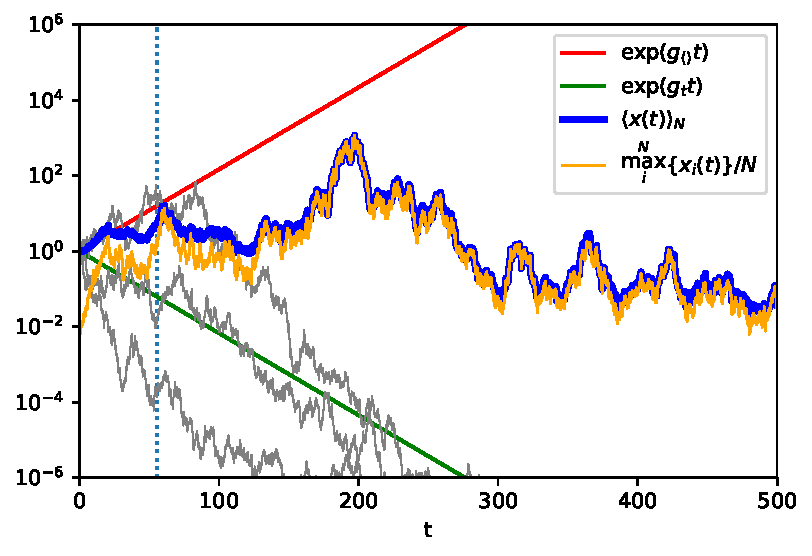
\includegraphics[height=9.3cm]{./chapter_3/figs/trajectories.pdf}
\caption{PEA and maximum in a finite ensemble of size $N=256$. {\bf \underline{Red line:}} expectation value $\ave{x(t)}$. 
{\bf \underline{Green line:}} exponential growth at the time-average growth rate. In the $T\to\infty$ limit all trajectories grow at this rate. 
{\bf \underline{Yellow line:}} contribution of the maximum value of any trajectory at time $t$ to the PEA.  
{\bf \underline{Blue line:}} PEA $\ave{x(t)}_N$.
{\bf \underline{Vertical line:}} Crossover -- for $t>t_c=\frac{2\ln N}{\sigma^2}$ the maximum begins to dominate the PEA (the yellow line approaches the blue line).
{\bf \underline{Grey lines:}} randomly chosen trajectories -- any typical trajectory soon grows at the time-average growth rate.  
{\bf \underline{Parameters:}} $N=256$, $\mu=0.05$, $\sigma=\sqrt{0.2}$.}
\flabel{trajectories}
\end{figure}
\FloatBarrier

\subsubsection{Our previous work on PEAs\seclabel{prevwork}}
In \cite{PetersKlein2013} we analysed PEAs of GBM analytically and numerically. Using \eref{GBM_sol} the PEA can be written as
\be
\ave{x}_N=\frac{1}{N} \sum_{i=1}^N \exp\left[ \left(\mu-\frac{\sigma^2}{2}\right) t + \sigma \gW_i(t) \right],
\elabel{PEA}
\ee
where $\left\{\gW_i(t)\right\}_{i=1\dots N}$ are $N$ independent realisations of the Wiener process. Taking the deterministic part out of the sum we re-write \eref{PEA} as
\be
\ave{x}_N=\exp\left[ \left(\mu-\frac{\sigma^2}{2}\right) t \right] \frac{1}{N} \sum_{i=1}^N \exp\left(t^{1/2} \sigma \xi_i\right),
\elabel{PEA_2}
\ee
where $\left\{\xi_i\right\}_{i=1\dots N}$ are $N$ independent standard normal variates.

We found that typical trajectories of PEAs grow at $\gex$ up to a time $t_c$ 
that is logarithmic in $N$, meaning $t_c\propto \ln N$. This is consistent with our sketch in \secref{sketch}. After this time, typical 
PEA-trajectories begin to deviate from expectation-value behavior, and eventually 
their growth rate converges to $g_t$. While the two limiting behaviours $N\to\infty$
and $t\to \infty$ can be computed exactly, what happens in between
is less straight-forward. The PEA is a random object outside these limits. 
In \cite{PetersKlein2013} we dealt with this issue numerically by creating a super-sample
of $S$ samples, each consisting of $N$ trajectories. In this way we were able to study the median of $\ave{x}_N(t)$, representing the behavior of typical trajectories.

A quantity of crucial interest to us is the exponential growth rate experienced by the PEA, 
\be
\gest(t,N) \equiv \frac{\ln(\ave{x(t)}_N)- \ln(x(0))}{t-0} = \frac{1}{t}\ln(\ave{x(t)}_N).
\elabel{gest}
\ee
In \cite{PetersKlein2013} we proved that the $t\to\infty$ limit for any (finite) 
$N$ is the same as for the case $N=1$, 
\be
\lim_{t\to\infty}\gest(t,N)=\mu-\frac{\sigma^2}{2}
\elabel{gest_2}
\ee
for all $N\geq1$. Substituting \eref{PEA_2} in \eref{gest} produces
\bea
\gest(t,N)&=&\mu-\frac{\sigma^2}{2}+\frac{1}{t} \ln\left(\frac{1}{N} \sum_{i=1}^N \exp( t^{1/2} \sigma \xi_i)\right)\\
&=&\mu-\frac{\sigma^2}{2}-\frac{\ln N}{t}+\frac{1}{t} \ln\left(\sum_{i=1}^N \exp( t^{1/2} \sigma \xi_i)\right).
\elabel{gest_4}
\eea

We didn't look in \cite{PetersKlein2013} at the expectation value of $\gest(t,N)$ for finite time and finite samples, but it's an interesting object that depends on $N$ and $t$ but is not stochastic. Note that this is not $\gest$ of the expectation value, 
which would be the $N\to\infty$ limit of \eref{gest}. Instead it is the 
$S\to\infty$ limit,
\be
\ave{\gest(t,N)} = \frac{1}{t}\ave{\ln(\ave{x(t)}_N)} = f(N,t),
\elabel{gest_3}
\ee
where, as in \secref{sketch}, $\ave{\cdot}$ without subscript refers to the average over all possible samples, \ie $\lim_{S\to\infty}\ave{\cdot}_{S}$. The last two terms in \eref{gest_4} suggest an exponential relationship between ensemble size and time. The final term is a tricky stochastic object on which the properties of the expectation value in \eref{gest_3} will hinge. This term will be the focus of our attention: the sum of exponentials of normal random variates or, equivalently, log-normal variates.


\subsubsection{Mapping to the random energy model}
Since the publication of \cite{PetersKlein2013} we have learned, thanks to discussions with J.-P.~Bouchaud, 
that the key object in \eref{gest_4} -- the sum of exponentials of normal random variates -- has been of
interest to the mathematical physics community since the 1980s. 

The reason for this is Derrida's random energy model \cite{Derrida1980,Derrida1981}. It is defined as follows. 
Imagine a system whose energy levels are $2^K=N$ random numbers $\xi_i$ (corresponding to $K=\ln N/\ln 2$ spins). This is
a very simple model of a disordered system, such as a spin glass, the idea being that the system is so complicated
that we ``give up'' and just model its energy levels as realizations of a random variable. (We denote the number 
of spins by $K$ and the number of resulting energy levels by $N$, whereas Derrida uses $N$ for the number of spins).
The partition function is then
\be
Z=\sum_{i=1}^N \exp\left(\beta J\sqrt{\frac{K}{2}}\xi_i\right),
\elabel{Z}
\ee
where the inverse temperature, $\beta$, is measured in appropriate units, and the scaling in $K$ is chosen
so as to ensure an extensive thermodynamic limit \cite[p.~79]{Derrida1980}. $J$ is a constant that will be determined below.
The logarithm of the partition function gives the Helmholtz free energy, 
\bea
F&=&-\frac{\ln Z}{\beta}\\
&=&-\frac{1}{\beta}  \ln\left[\sum_{i=1}^N \exp\left(\beta J \sqrt{\frac{K}{2}}\xi_i\right)\right].
\elabel{F}
\eea

Like the growth rate estimator in \eref{gest}, this involves a sum of 
log-normal variates and, indeed, we can rewrite \eref{gest_4} as
\be
\gest=\mu-\frac{\sigma^2}{2}-\frac{\ln N}{t}-\frac{\beta F}{t},
\elabel{gest_5}
\ee
which is valid provided that
\be
\beta J \sqrt{\frac{K}{2}}=\sigma t^{1/2}.
\elabel{map}
\ee
\Eref{map} does not give a unique mapping between the parameters of our GBM, $(\sigma, t)$, and the parameters of the REM, $(\beta, K, J)$. Equating (up to multiplication) the constant parameters, $\sigma$ and $J$, in each model gives us a specific mapping:
\be
\sigma=\frac{J}{\sqrt{2}} \quad \text{and} \quad t^{1/2} = \beta\sqrt{K}.
\elabel{choice_1}
\ee



The expectation value of $\gest$ is interesting. The only random object
in \eref{gest_5} is $F$. Knowing $\ave{F}$ thus amounts to knowing $\ave{\gest}$.
In the statistical mechanics of the random energy model $\ave{F}$ is of key
interest and so much about it is known. We can use this knowledge
thanks to the mapping between the two problems.

Derrida identifies a critical temperature,
\be
\frac{1}{\beta_c} \equiv \frac{J}{2\sqrt{\ln 2}},
\elabel{beta_c}
\ee
above and below which the expected free energy scales differently with $K$ and $\beta$. This maps to a critical time scale in GBM,
\be
t_c = \frac{2\ln N}{\sigma^2},
\elabel{t_c}
\ee
with high temperature ($1/\beta>1/\beta_c$) corresponding to short time ($t<t_c$) and low temperature ($1/\beta<1/\beta_c$) corresponding to long time ($t>t_c$). Note that $t_c$ in \eref{t_c} scales identically with $N$ and $\sigma$ as the transition time, \eref{short_t}, in our sketch.

In \cite{Derrida1980}, $\ave{F}$ is computed in the high-temperature (short-time) regime as
\bea
\ave{F}&=&E-S/\beta \\
&=&-\frac{K}{\beta} \ln2 - \frac{\beta K J^2}{4},
\elabel{F_2}
\eea
and in the low-temperatures (long-time) regime as
\be
\ave{F}=-KJ\sqrt{\ln 2}.
\elabel{F_3}
\ee

\underline{Short time}\\
We look at the short-time behavior first (high $1/\beta$, \eref{F_2}).
The relevant computation of the entropy $S$ in \cite{Derrida1980} 
involves replacing the number of energy levels
$n(E)$ by its expectation value $\ave{n(E)}$. This is justified because
the standard deviation of this number is $\sqrt{n}$ and relatively small
when $\ave{n(E)}>1$, which is the interesting regime in Derrida's case. 

For spin glasses, the expectation value of $F$ is interesting, supposedly, 
because the system may be self-averaging and can be thought of as an
ensemble of many 
smaller sub-systems that are essentially independent. The macroscopic
behavior is then given by the expectation value.

Taking expectation values and substituting from \eref{F_2} in \eref{gest_5} we find
\be
\ave{\gest}^{\text{short}}=\mu-\frac{\sigma^2}{2}+\frac{1}{t} \frac{K J^2}{4T^2}.
\elabel{gest_6}
\ee
From \eref{map} we know that $t=\frac{KJ^2}{2\sigma^2T^2}$, which we substitute, to find
\be
\ave{\gest}^{\text{short}}=\mu,
\elabel{gest_7}
\ee
which is the correct behavior in the short-time regime.

\underline{Long time}\\
Next, we turn to the expression for the long-time regime (low temperature, \eref{F_3}). 
Again 
taking expectation values and substituting, this time from \eref{F_3} in \eref{gest_5}, we find
for long times
\be
\ave{\gest}^{\text{long}}=\mu-\frac{\sigma^2}{2}-\frac{\ln{N}}{t}+\sqrt{\frac{2\ln N}{t}}\,\sigma,
\elabel{gest_8}
\ee
which has the correct long-time asymptotic behavior.
The form of the correction to the time-average growth rate
in \eref{gest_8} is consistent with \cite{PetersKlein2013} and \cite{Redner1990}, where
it was found that approximately $N=\exp(t)$ systems are required for ensemble-average
behavior to be observed for a time $t$, so that the parameter $\ln N/t$ controls
which regime dominates -- if the parameter is small, then \eref{gest_8} indicates that the
long-time regime is relevant.

\Fref{1} is a direct comparison between the results derived
here, based on \cite{Derrida1980}, and numerical results using the same parameter 
values as in \cite{PetersKlein2013}, namely $\mu=0.05, \sigma=\sqrt{0.2}, N=256$ and $S=10^5$.


Notice that $\ave{\gest}$ is not the (local)
time derivative $\frac{\partial}{\partial t}\ave{\ln(\ave{x}_N)}$, but a time-average growth rate, $\ave{\frac{1}{t}\ln\left( \frac{\ave{x(t)}_N}{\ave{x(0)}_N}\right)}$. 
In \cite{PetersKlein2013} we used a notation that we've stopped using since then because it
caused confusion -- $\ave{g}$ there denotes the growth rate of the expectation value, which 
is not the expectation value of the growth rate. 



It is remarkable that the expectation value $\ave{\gest(N,t)}$ so closely reflects the
median, $q_{0.5}$, of $\ave{x}_N$, in the sense that
\be
q_{0.5}(\ave{x(t)}_N) \approx \exp \left(\ave{\gest(N,t)}t\right).
\elabel{quant_ave}
\ee
In \cite{PetersGell-Mann2016} it was discussed in detail that 
$\gest(1,t)$ is an ergodic observable for \eref{GBM}, in the sense that 
$\ave{\gest(1,t)}=\lim_{t\to\infty} \gest$. The relationship in \eref{quant_ave}
is far more subtle. The typical behavior of GBM PEAs 
is complicated outside the limits $N\to\infty$ or $t\to\infty$, in the sense that growth rates are 
time dependent here. This complicated behavior is well represented by an 
approximation that uses physical insights into spin glasses. Beautiful!

\begin{figure}
\centering
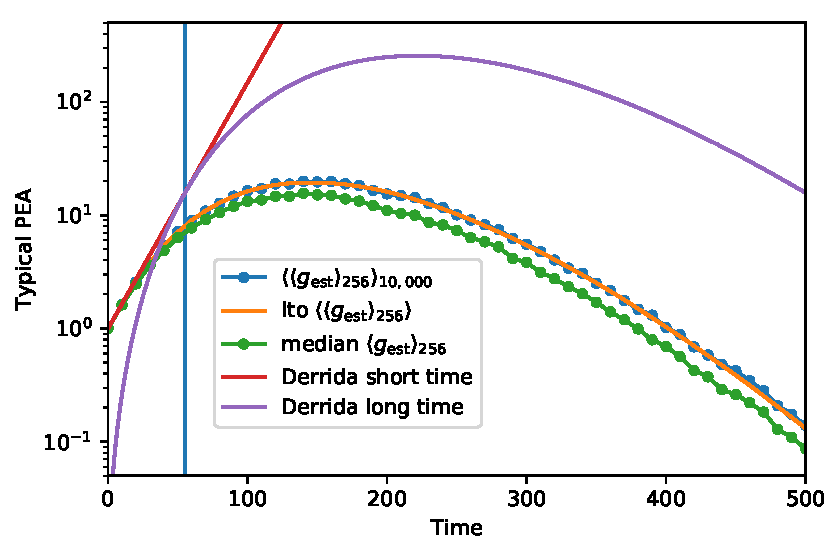
\includegraphics[height=9.3cm]{./chapter_3/figs/PEA.pdf}
\caption{Lines are obtained by exponentiating the various exponential 
growth rates. {\bf \underline{Blue line:}} $\ave{\ave{\gest}_{256}}_{10,000}$ is the numerical mean 
(approximation of the expectation value) 
over a super-ensemble of $S=10,000$ samples of $\gest$ estimated in sub-ensembles of $N=256$ GBMs each. 
{\bf \underline{Green line:}} median in a super-ensemble of $S$ samples of $\gest$, each estimated in sub-ensembles of size $N$. 
{\bf \underline{Yellow line:}} \eref{Ito_sums} is an exact expression for $d\ave{\ln\ave{x}_N}$, derived using \Ito calculus. We evaluate the expression by Monte Carlo, and integrate, $\ave{\ln\ave{x}_N}=\int_{0}^{t} d\ave{\ln\ave{x}_N}$. Exponentiation yields the yellow line. 
{\bf \underline{Red line:}} short-time behavior, based on the random energy model, \eref{gest_7}.
{\bf \underline{Purple line:}} long-time behavior, based on the random energy model, \eref{gest_8}. {\bf \underline{Vertical line:}} Crossover between the regimes at $t_c=\frac{2\ln N}{\sigma^2}$, corresponding to $\beta_c=\frac{2(\ln 2)^{1/2}}{J}$.
{\bf \underline{Parameters:}} $N=256$, $S=10,000$, $\mu=0.05$, $\sigma=\sqrt{0.2}$.}
\flabel{1}
\end{figure}
\FloatBarrier
%

\subsubsection{Another route via \Ito calculus}
Another way to find the expectation value of PEA growth rates, \eref{gest_3}, 
is to compute $\ave{d\ln \ave{x}_N}$ using \Ito calculus. We compute this directly, without 
invoking the random energy model. To apply \Ito calculus, 
we will need the first two partial derivatives of $d\ln\ave{x}_N$ with respect to $x_i$.
\be
\frac{\partial \ln \ave{x}_N}{\partial x_i}=\frac{1}{N\ave{x}_N}
\ee
and
\be
\frac{\partial^2 \ln \ave{x}_N}{\partial x_i^2}=-\frac{1}{N^2\ave{x}_N^2}
\ee
Now, Taylor-expanding $d \ln \ave{x}_N$ we find
\bea
d \ln \ave{x}_N&=&\sum_i \frac{\partial \ln \ave{x}_N}{\partial x_i} dx_i+\frac{1}{2}\sum_i \sum_j \frac{\partial^2 \ln \ave{x}_N}{\partial x_i \partial x_j} dx_i dx_j+ \ldots\\
&\approx&\frac{1}{N\ave{x}_N} \sum_i dx_i-\frac{1}{2N^2\ave{x}_N^2}\sum_i \sum_j dx_i dx_j.
\eea
The double-sum can be split into `diagonal' ($i=j$) terms and cross-terms as
\be
\frac{1}{N\ave{x}_N}\sum_i x_i(\mu dt + \sigma dW_i) -\frac{1}{2N^2\ave{x}_N^2 }\left(\sum_i  dx_i^2 + \sum_{j}\sum_{i \neq j}dx_i dx_j\right)\hspace{.6cm}
\ee
Parts of the cross-terms are negligible because they are of order $dt^2$ and the rest vanishes when taking the expectation value, 
as we see by writing out one cross term
\be
dx_i dx_j=x_i x_j (\mu^2 dt^2+\mu\sigma dt dW_i+\mu \sigma dt dW_j + \sigma^2 dW_i dW_j).
\ee
We therefore drop these terms now, as we take the expectation value, using the Wiener identity $\ave{dW_i^2}=dt$ for the final term
\bea
\ave{d \ln \ave{x}_N}&=&\ave{\mu dt -\frac{1}{2N^2\ave{x}_N^2}\sum_i x_i^2 (\mu^2 dt^2 + \sigma^2 dt)} \\
&=&\mu dt   -\ave{\frac{1}{2} \sigma^2 \frac{\ave{x^2}_N}{N\ave{x}_N^2}} dt + O(dt^2).
\eea
Discarding terms of higher-than-first order in $dt$ and re-writing the last term as a fraction of sums, we thus have 
\bea
\frac{\ave{d \ln \ave{x}_N}}{dt}&=&\mu -\frac{1}{2} \sigma^2  \ave{\frac{\frac{1}{N}\sum_i x_i^2}{N\left(\frac{1}{N}\sum_i x_i\right)^2}}  \\
&=&\mu -\frac{1}{2} \sigma^2  \ave{\frac{\sum_i x_i^2}{\left(\sum_i x_i\right)^2}} \elabel{Ito_sums}
\eea
This expression has the correct behaviour: for short times, all $x_i$ are essentially identical, 
and the second term is $-\frac{1}{2}\sigma^2 \frac{1}{N}$, which is negligible if $N$ is large. So, for short times
we see expectation-value behaviour. For long times, the largest $x_i$ will dominate both the numerator and the denominator, and we have
$-\frac{1}{2}\sigma^2$: the full \Ito correction is felt for long times.

\subsubsection{Discussion}
The \Ito result is exact. A Monte-Carlo estimate of \eref{Ito_sums} (which is easy to obtain) is 
shown in \fref{1} (yellow line). This agrees well with numerical observations.
The approximations from the random energy model have the right shape and asymptotic behavior, 
though they're not on the same scale as the median PEA. This is, of course, not surprising because
these estimates are not designed to coincide with the median PEA. Quantitatively they are closer to 
a higher quantile of the distribution of PEAs. An intriguing question is this: is our computation 
using \Ito calculus helpful to compute the expected free energy of the random energy model? 

\subsection{Cooperation}
\seclabel{Cooperation}
Under multiplicative growth, fluctuations are undesirable because they reduce 
time-average growth rates. In the long run, wealth $x_1(t)$ with noise term 
$\sigma_1$ will outperform wealth $x_2(t)$ with a larger 
noise term $\sigma_2>\sigma_1$, in the sense that 
\be
\gt(x_1) > \gt(x_2)
\ee
with probability 1.

For this reason it is desirable to reduce fluctuations. One protocol that achieves this is 
resource pooling and sharing. In \secref{Every_man} we explored the world created 
by the model of independent GBMs. This is a world where everyone experiences the 
same long-term growth rate. We want to explore the effect of the invention of 
cooperation. As it turns out cooperation increases growth rates, and this is a 
crucial insight. 

Suppose two individuals, $x_1(t)$ and $x_2(t)$ decide to meet up every Monday, put all 
their wealth on a table, divide it in two equal amounts, and go back to their business, \ie
they submit their wealth to our toy dynamic \eref{GBM}. How 
would this operation affect the dynamic of the wealth of these two individuals?

 Consider a discretized version of \eref{GBM}, such as would be used in a numerical simulation. The non-cooperators grow according to
 \bea
 \d x_i(t) & = & x_i(t) \left[\mu \dt + \sigma \sqrt{\dt}\,\xi_i\right], \elabel{discrete_nonc_grow} \\
 x_i(t+\dt) & = & x_i(t) + \d x_i(t), \elabel{discrete_nonc_coop}
 \eea
 where $\xi_i$ are standard normal random variates, $\xi_i\sim \mathcal{N}(0,1)$.

We imagine that the two previously non-cooperating entities, with resources $x_1(t)$ and $x_2(t)$, cooperate to produce two entities, whose resources we label $x^c_1(t)$ and $x^c_2(t)$ to distinguish them from the non-cooperating case. We envisage equal sharing of resources, $x^c_1=x^c_2$, and introduce a cooperation operator, $\oplus$, such that
 \be
 x_1 \oplus x_2 = x^c_1 + x^c_2.
 \ee
 
 In the discrete-time picture, each time step involves a two-phase process. First there is a growth phase, analogous to \eref{GBM}, in which each cooperator increases its resources by
 \be
 \d x^c_i(t) = x^c_i(t)\left[\mu\dt + \sigma\sqrt{\dt}\,\xi_i\right].
 \elabel{discrete_coop_grow}
 \ee
 This is followed by a cooperation phase, replacing \eref{discrete_nonc_coop}, in which resources are pooled and shared equally among the cooperators:
 \be
 x^c_i(t+\dt) = \frac{ x^c_1(t) + \d x^c_1(t) + x^c_2(t) + \d x^c_2(t)}{2}.
 \elabel{discrete_coop_coop}
 \ee
 
 \begin{figure}
 \centering
 \begin{picture}(300,230)(60,0)
 \put(-20,0){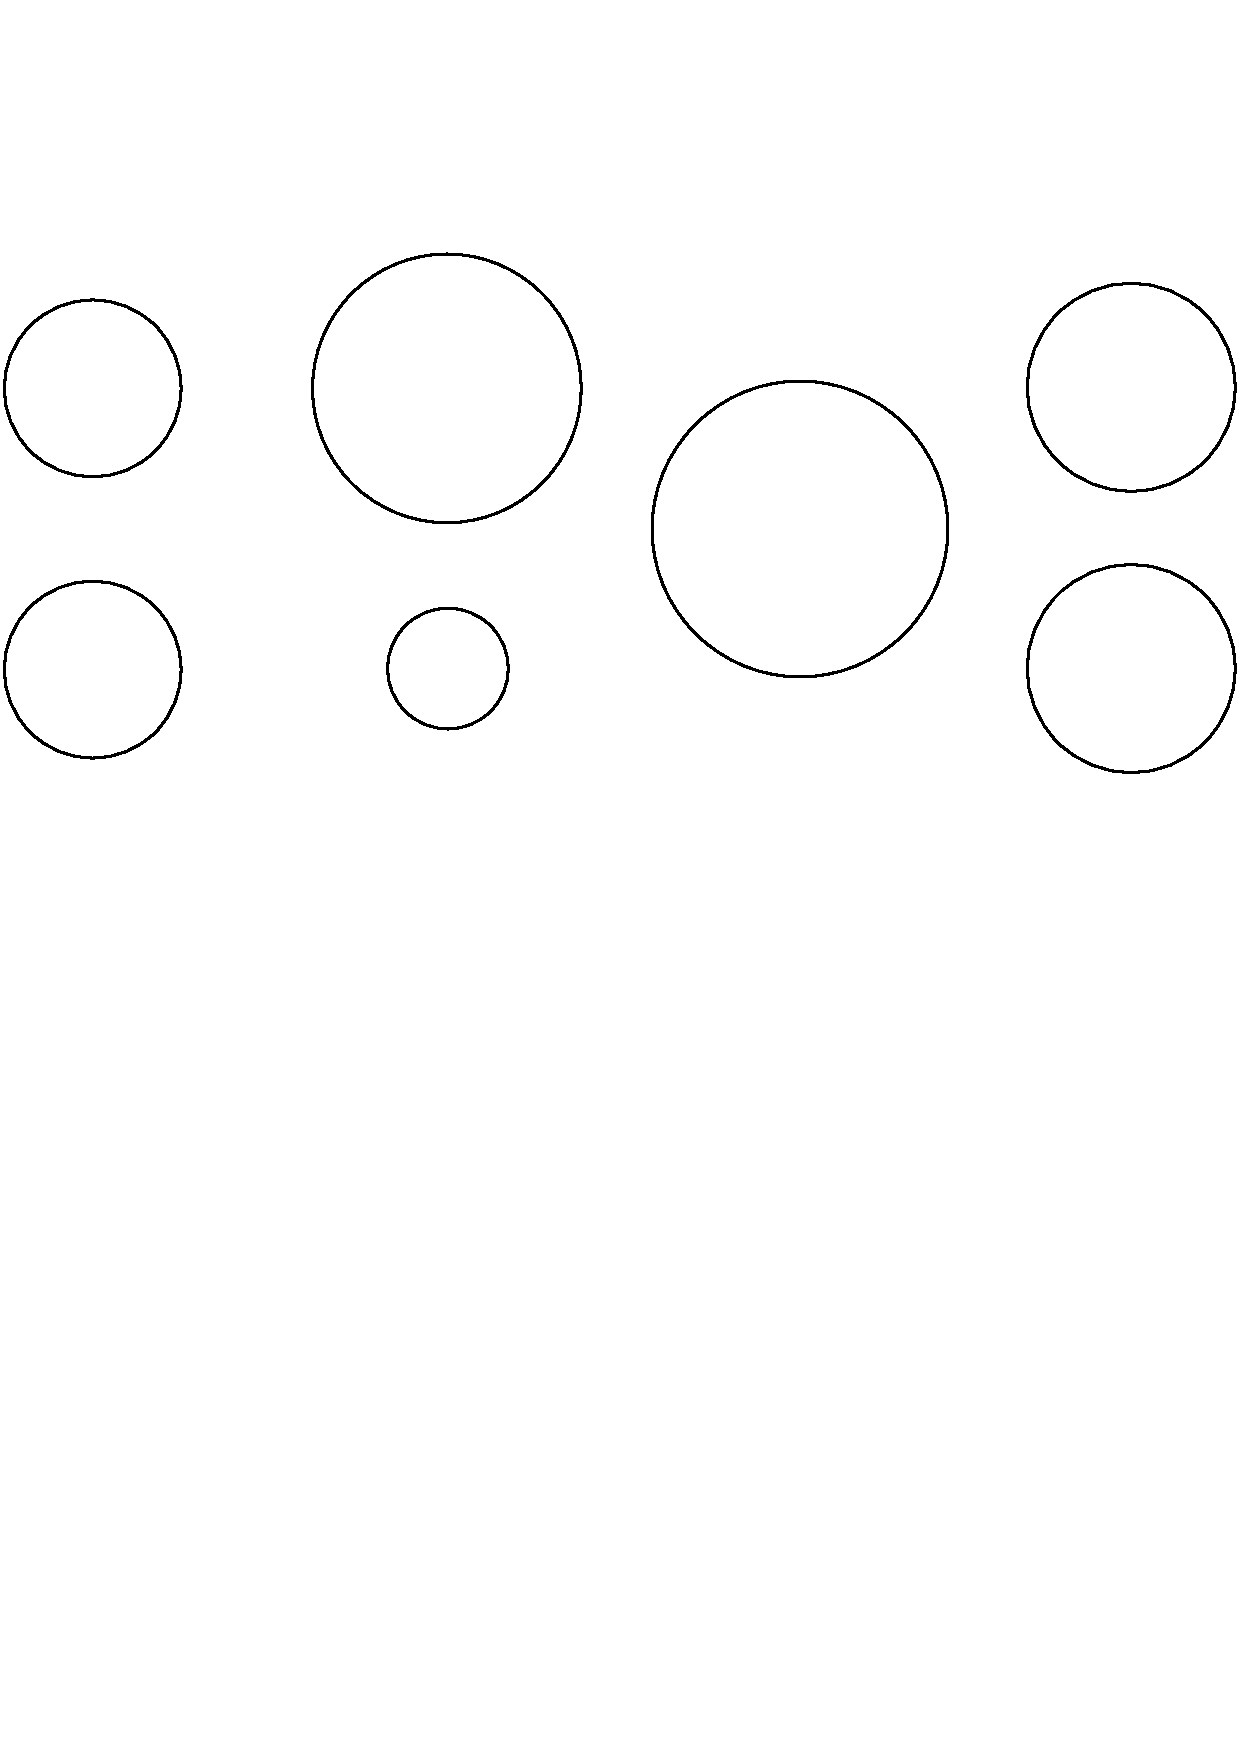
\includegraphics[width=470pt]{./chapter_3/figs/blobs.pdf}}
 \put(0,145){$x^c_1(t)$}
 \put(48,147){\vector(1,0){45}}
 \put(0,40){$x^c_2(t)$}
 \put(48,40){\vector(1,0){75}}
 %
 \put(115,145){$x^c_1(t)+\d x^c_1(t)$}
 \put(200,147){\vector(3,-2){30}}
 \put(138,46){$x^c_2(t)$}
 \put(130,34){$+\d x^c_2(t)$}
 \put(173,45){\vector(3,2){50}}
 %
 \put(255,100){$x^c_1(t)+\d x^c_1(t)$}
 %
 \put(250,85){$+ x^c_2(t)+\d x^c_2(t)$}
 \put(335,75){\vector(3,-2){30}}
 \put(335,117){\vector(3,2){30}}
 %
 \put(385,145){$x^c_1(t+\dt)$}
 \put(385,40){$x^c_2(t+\dt)$}
 %
 \put(448,147){\vector(1,0){25}}
 \put(448,40){\vector(1,0){25}}

 \put(476,144.5){$\cdots$}
 \put(476,37.5){$\cdots$}
 % AA extra arrows
 \put(-47,117){\vector(3,2){25}}
 \put(-47,75){\vector(3,-2){25}}
 \put(-62,114){$\cdots$}
 \put(-62,73){$\cdots$}
 %
 \put(50,207.5){\large{Grow}}

 \put(215,190){$\overbrace{\text{Pool} \hspace{3cm}\text{Share}}^{\text{\large{Cooperate}}}$}

 \end{picture}
 \caption{Cooperation dynamics. Cooperators start each time step with equal resources, then they {\it grow} independently 
 according to \eref{discrete_coop_grow}, then they {\it cooperate} by {\it pooling} resources and {\it sharing} them equally, 
 then the next time step begins. 
  }
 \flabel{dynamics}
 \end{figure}
 

 %Analysis
 With this prescription both cooperators and their sum experience the following dynamic:
 \be
 (x_1 \oplus x_2)(t+\dt) =
 (x_1 \oplus x_2)(t) \left[1 + \left(\mu \dt + \sigma \sqrt{\dt} \, \frac{\xi_1 + \xi_2}{2}\right)\right].
 \elabel{discrete_cooperate}
 \ee
 For ease of notation we define
 \be
 \xi_{1\oplus2}=\frac{\xi_1+\xi_2}{\sqrt{2}},
 \ee
 which is another standard Gaussian, $\xi_{1\oplus2} \sim \mathcal{N}(0,1)$. Letting the time
 increment $\dt \to 0$ we recover an equation of the same form as
 \eref{GBM} but with a different fluctuation amplitude,
 \begin{equation}
 d(x_1 \oplus x_2) = (x_1 \oplus x_2)\left(\mu dt +\frac{\sigma}{\sqrt{2}} dW_{1\oplus2}\right).
 \end{equation}
 
The expectation values of a non-cooperator, $\ave{x_1(t)}$, and a corresponding cooperator,
$\ave{x^c_1(t)}$, are identical. Based on expectation values, we thus cannot 
 see any benefit of cooperation. Worse still, immediately after the growth phase, the 
 better-off entity of a cooperating pair, $x^c_1(t_0)>x^c_2(t_0)$, say, would increase its expectation value from 
$\frac{x^c_1(t_0)+x^c_2(t_0)}{2}\exp(\mu (t-t_0))$ to $x^c_1(t_0)\exp(\mu (t-t_0))$
by breaking the cooperation. But it would be foolish to act on the basis of this analysis --
the short-term gain from breaking cooperation is a one-off, and is dwarfed by the long-term
multiplicative advantage of continued cooperation. 
An analysis based on expectation values finds that there is no reason for 
cooperation to arise, and that if it does arise there are good reasons for it to end, 
\ie it will be fragile. Because expectation values are inappropriately used to evaluate 
future prospects, the observation of widespread cooperation constitutes a conundrum. 

%Solution of the cooperation conundrum
The solution of the conundrum comes from considering the time-average
growth rate. The non-cooperating entities grow at $g_{t}(x_i)=\mu-\frac{\sigma^2}{2}$, 
whereas the cooperating unit benefits from a reduction of the amplitude of relative 
fluctuations and grows at $g_{t}(x_1\oplus x_2)=\mu-\frac{\sigma^2}{4}$, 
and we have
\begin{equation}
g_{t}(x_1\oplus x_2)>g_{t}(x_i)
\end{equation}
for any non-zero noise amplitude. Imagine a world where cooperation does not exist, 
just like in \secref{Every_man}. Now introduce into this world two individuals who have 
invented cooperation -- very quickly this pair of individuals will be vastly more wealthy than
anyone else. To keep up, others will have to start cooperating. The effect is illustrated 
in \fref{cooperate} by direct simulation of
\eref{discrete_nonc_grow}--\eref{discrete_nonc_coop} and \eref{discrete_cooperate}.

\begin{figure}
\begin{picture}(200,300)(0,0)
\put(-35,-135){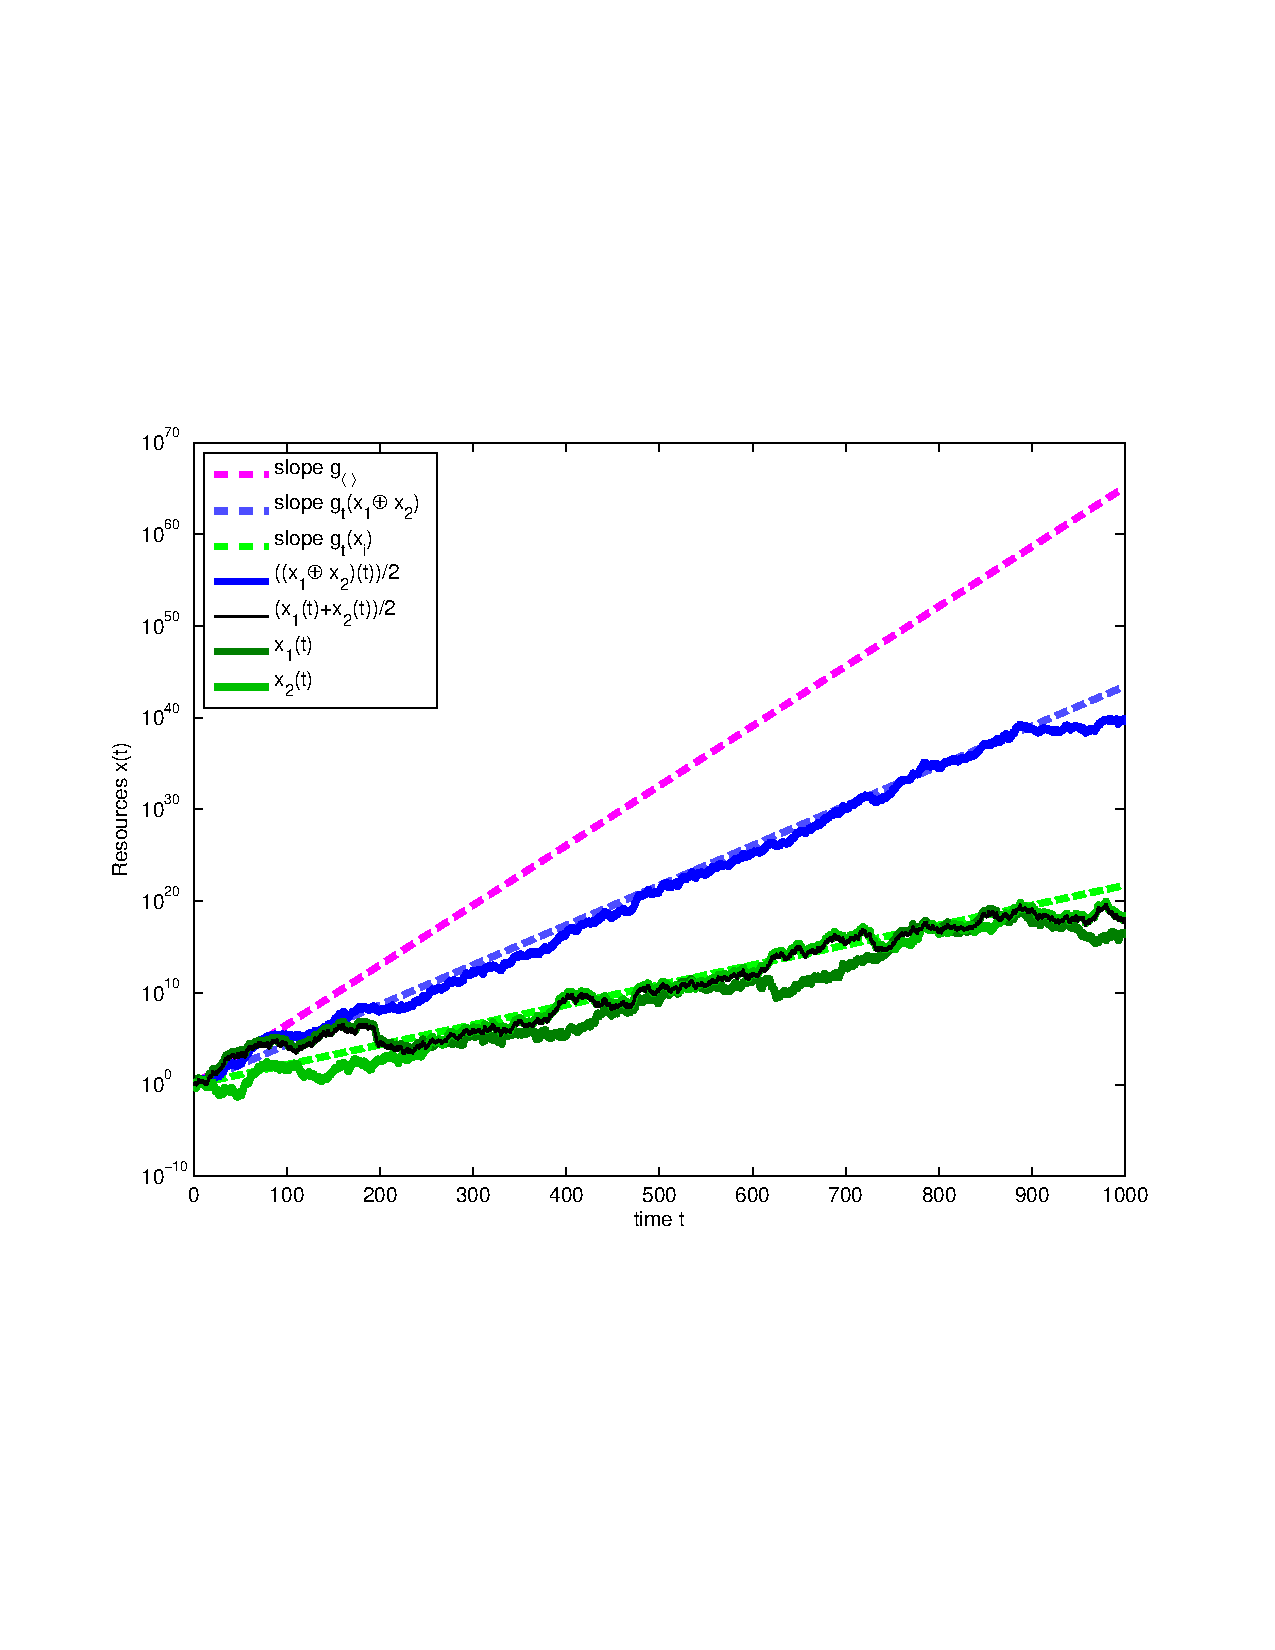
\includegraphics[width=440pt]{./chapter_3/figs/cooperate.pdf}}
\end{picture}
\caption{Typical trajectories for two non-cooperating (green) entities and for the 
corresponding cooperating unit (blue).
Over time, the noise reduction for the cooperator leads to faster growth. Even without
effects of specialisation or the emergence of new function, 
cooperation pays in the long run. The black thin line shows the average of the 
non-cooperating entities. While in the logarithmic vertical scale the average traces
the more successful trajectory, it is far inferior to the cooperating unit. 
In a very literal mathematical sense the whole, $(x_1 \oplus x_2)(t)$, is more than the sum of its
parts, $x_1(t)+x_2(t)$. The algebra of cooperation is not merely that of summation.}
\flabel{cooperate}
\end{figure}

Imagine again the pair of cooperators outperforming all of their peers. Other
entities will have to form pairs to keep up, and the obvious next step is for larger
cooperating units to form -- groups of 3 may form, pairs of pairs, cooperation 
clusters of $n$ individuals, and the larger the cooperating group the closer the
time-average growth rate will get to the expectation value.
For $n$ cooperators, $x_1\oplus x_2 ... \oplus x_n$ the spurious drift term is 
$-\frac{\sigma^2}{2n}$, so that the time-average growth approaches 
expectation-value growth for large $n$. The approach to this upper bound as 
the number of cooperators increases favours the formation of social structure. 

We may generalise to different drift 
terms, $\mu_i$, and noise amplitudes, $\sigma_i$, for different individual entities. 
Whether cooperation is beneficial in the long run for any
given entity depends on these parameters as follows. Entity 1 
will benefit from cooperation with entity 2 if 
\be
\mu_1-\frac{\sigma_1^2}{2}<\frac{\mu_1+\mu_2}{2}-\frac{\sigma_1^2+\sigma_2^2}{8}.
\ee
We emphasize that this inequality may be satisfied also if the expectation value
of entity 1 grows faster than the expectation value of entity 2, \ie if
$\mu_1>\mu_2$. An analysis of expectation values, again, is utterly misleading:
the benefit conferred on entity 1 due to the fluctuation-reducing effect of 
cooperation may outweigh the cost of having to cooperate with an entity with
smaller expectation value.
 
Notice the nature of the Monte-Carlo simulation in \fref{cooperate}. No ensemble
is constructed. Only individual trajectories are simulated and run for a time that is 
long enough for statistically significant features to rise above the noise. This method
teases out of the dynamics what happens over time. The significance of any observed 
structure -- its epistemological meaning -- is immediately clear: this is what happens over time
for an individual system (a cell, a person's wealth, {\it etc.}). Simulating an ensemble
and averaging over members to remove noise does not tell the same story. The resulting
features may not emerge over time. They are what happens on average in an ensemble, 
but -- at least for GBM -- this is not what happens to the individual with probability 1. For instance the 
 pink dashed line in \fref{cooperate} is the ensemble average of $x_1(t)$, $x_1(t)$, 
 and $(x_1 \oplus x_2)(t)/2$, and it has nothing to do with what happens 
 in the individual trajectories over time.

When judged on expectation values, the apparent futility of cooperation is unsurprising
because expectation values are the result for infinitely 
many cooperators, and adding further cooperators cannot improve on this.

In our model the advantage of cooperation, and hence the emergence
of social structure in the broadest sense -- is purely a non-linear 
effect of fluctuations -- cooperation reduces the magnitude of 
fluctuations, and over time (though not in expectation) this implies faster growth. 


Another generalisation is partial cooperation -- entities may share only
a proportion of their resources, resembling taxation and redistribution. We discuss this in
the next section.
\FloatBarrier

\subsection{Reallocation}\label{reallocation}

\subsubsection{Introduction}\label{sec:introduction}

% What is the EH and why is it made?
%%Indeed, Samuelson wrote that, by adopting it, theorists had hoped to avoid taking economics ``out of the realm of science into the realm of genuine history''~\cite[p.~12] {Samuelson1968}.
Paul Samuelson identified the ``ergodic hypothesis'' in the mindset of classical economic theorists, defining it as ``a belief in unique long-run equilibrium independent of initial conditions''~\cite[pp.~11-12]{Samuelson1968}. Classically, the equilibrium is studied and the transient phenomena preceding it are ignored. This approach simplifies analysis greatly and is widespread. Here we present an empirical test of the validity of the ergodic hypothesis as applied to the distribution of wealth. We find it inconsistent with historical data from the United States (US), raising doubts about the conclusions of studies in which it is made.

% Transformation is needed
Economics is often concerned with growth. A growing quantity cannot be ergodic in Samuelson's sense because it does not tend to an equilibrium value. Na\"ively, then, the ergodic hypothesis seems an inappropriate modelling choice in this context, ruling out a swathe of analytical techniques. Although this is rarely stated explicitly, a common strategy to salvage these techniques is the following: find a transformation of the non-ergodic process that produces a meaningful ergodic observable. 
If such an ergodic observable can be derived, then classical techniques may still be useful. For instance,~\cite{PetersGell-Mann2016} show that utility theory can be viewed as an attempt to transform non-ergodic growing wealth into ergodic growth rates. Expectation values -- which would otherwise be misleading -- then quantify time-average growth of the decision-maker's wealth.
%\ie utility changes can be ergodic even if the underlying wealth process is not. [AA deleted. Let's say what classical technique this resurrects.]

% This is done in studies of wealth distributions
Studies of wealth distributions also employ this strategy. Individual wealth is modelled as a growing quantity. Dividing by the population average transforms this to a rescaled wealth, which is hypothesised to be ergodic. Formally, the distribution of the stochastic process for the rescaled wealth is assumed to converge to a unique and time-independent distribution. For example,~\cite{BenhabibBisinZhu2011} ``impose assumptions [\ldots] that guarantee the existence and uniqueness of a limit stationary distribution'' (p.~130). Similar formulations appear in~\cite{stiglitz1969distribution,bewley1977permanent,piketty2013theory,de2015quantitative,de2015piketty,jones2015pareto}. These studies take advantage of the simplicity with which the stationary distribution can then be analyzed, \eg to test the effects of policies encoded in model parameters.

Treating the stationary model distribution as representative of the empirical wealth distribution implies an assumption of fast convergence, \ie that the actual distribution approaches its asymptotic form on a timescale shorter than that of relevant changes in economic conditions. For example, the top rate of income tax in the US was reduced from 91 percent to 70 percent between 1963 and 1965. The next change occurred about 20 years later, in 1982, when it was reduced to 50 percent. In this example, convergence would be fast if the model distribution were close to its asymptotic form after, say, 5 years. Convergence would be slow if this took, say, 100 years.~\cite[p.~137] {atkinson1969timescale} argued that ``the speed of convergence makes a great deal of difference to the way in which we think about the model''. It determines the practical relevance of the stationary distribution~\cite{atkinson1969timescale,cowell2014piketty}.

% Other models
Recent research has marked a shift away from studying the stationary distribution in isolation.~\cite{gabaix2015dynamics,BermanBen-JacobShapira2016,kaymak2016evolution,berman2017revisiting} study the dynamics of wealth and income, rather than how they are distributed asymptotically. Some of these studies also consider convergence times~\cite{gabaix2015dynamics,berman2017revisiting}.

% What is the problem? What are we going to do?
There is, however, an elephant in the room. To our knowledge, the validity of the ergodic hypothesis for rescaled wealth has never been tested empirically. Here we present such a test. For the test to be meaningful, a model is required that does not assume ergodicity from the outset. It must have regions of parameter space (``regimes'') in which the ergodic hypothesis for rescaled wealth does and does not hold.
%As ergodicity depends on dynamics, the test cannot be carried out by looking at a wealth distribution in isolation. Instead, the dynamics of wealth must be considered.

% Our model
% AA20170120 - introduced reallocation here to make subsequent comments understandable
Our model satisfies this condition. Its basis is that individual wealth undergoes noisy exponential growth. Social structure is represented by a wealth reallocation mechanism in which a fraction of everyone's wealth is pooled and shared. The sign of the reallocation rate parameter determines whether a stationary distribution exists: if positive (corresponding to reallocation from richer to poorer) then it does; if negative (from poorer to richer) then it doesn't.

We estimate model parameters using three different datasets of historical wealth shares in the US population. These estimated parameters -- and not an {\it a priori} assumption -- tell us whether a stationary distribution exists. When it does, it has a Pareto tail, consistent with data and standard models~\cite{Pareto1897,DragulescuYakovenko2001}. We evaluate convergence times, when convergence is possible, to assess whether the ergodic hypothesis is acceptable in practice.

%Our results
% AA20170120 - added comment on negative reallocation
Our findings invalidate the ergodic hypothesis. The fitted reallocation rate is not robustly positive for any dataset we analyze. Indeed, for one dataset we find it to be consistently negative for the last thirty years or so. We cannot overstate our surprise at this finding. Most theorists would consider a model in which individual wealths grow independently, \ie with no reallocation, an extreme and unrealistic model of an advanced Western economy with socio-political institutions and infrastructure. We would expect to infer consistent positive reallocation from data for such an economy. We find the opposite: that, from the 1980s to the present, the US economy is best described in our model as one in which wealth is systematically reallocated from poorer to richer.

% AA20170120 - merged sentence from last para and added remark on negative reallocation
Other datasets yield reallocation rates for which a stationary distribution does exist, but with convergence times of decades or centuries. Whichever data are used, our analysis does not provide the unequivocal endorsement of the ergodic hypothesis that would justify its ubiquitous use in the field. Policy recommendations based on models which assume the existence of a stationary distribution and fast convergence may be ineffective in practice. Worse still, such inappropriately-constrained models may paint a misleading picture of reality, for example that with taxation and public spending our economies are positively redistributive. This could lead to policy prescriptions which run counter to policy goals.

% earnings
We also extend our model to treat explicitly additive changes in wealth, akin to labor income and consumption. This allows us to answer the question whether rescaled wealth is inherently unstable, or whether it is inherently stable with increases in its inequality driven by increasingly unequal earnings. We find that earnings had only a small effect on the dynamics of the wealth distribution over the last century
% -- we suspect due to a high wealth-to-income ratio -- 
and that changes in their distribution do not explain adequately the observed instability in wealth.

Our contribution is threefold. Firstly, we develop a theoretical model which describes the dynamics of wealth and allows us to test empirically the validity of the ergodic hypothesis. Naturally, this cannot be done using models in which the ergodic hypothesis is implicit.

Secondly, we use the model to assess how fast the wealth distribution converges to its asymptotic form, when this exists. We find convergence times greater than the typical intervals between changes in policy and other determinants of the distribution. This casts doubt over the ability of models with fast convergence to interpret observed changes in inequality and yield effective policy.

%Thirdly, our study contributes to a body of work examining ergodicity in economic systems. Indiscriminate use of the ergodic hypothesis can mean that non-ergodic processes are analyzed with methods appropriate only for ergodic processes. This is a severe methodological problem and it has been argued that this mismatch is behind open problems in economics~\cite{Peters2011b}. This study demonstrates the importance of establishing empirically and analytically which observables may legitimately be treated as ergodic.

Thirdly, our study extends a body of theory of economic systems without assuming ergodicity.~\cite{PetersGell-Mann2016} show that a sound decision theory can be developed by finding ergodic growth rates for non-ergodic wealth processes. In the present context,~\cite{AdamouPeters2016} derive a fundamental measure of wealth inequality from such growth rates. Elsewhere,~\cite{Peters2011b} resolves the St.~Petersburg paradox by maximizing individual performance over time and~\cite{Peters2011a} applies the same reasoning to derive an optimal leverage for stock-market investments.~\cite{PetersAdamou2013} extend this work to derive constraints on price fluctuations in freely-traded assets, resolving the equity premium puzzle of~\cite{MehraPrescott1985}.

Indiscriminate use of the ergodic hypothesis can mean that non-ergodic processes are analyzed with methods appropriate only for ergodic processes. This is a severe methodological problem, which we argue is behind many open problems in economics. Our work demonstrates the importance of establishing empirically and analytically which observables may be treated legitimately as ergodic.

%Thirdly, we find that the three analyzed US wealth datasets differ in their implications regarding ergodicity. This highlights the importance of the debate about the measurement of top wealth shares in the United States~\cite{kopczuk2015we,bricker2016measuring}.
%OP deleted statement that different conclusions about ergodicity come out of the different datasets. I know what we meant by that, but it's muddling the message. None of the datasets supports the ergodic hypothesis because none of them says there couldn't possibly be a problem with it.

%\OP{What about the fact that prevailing conditions look like they're pushing people into negative wealth and destroy the middle class? Ergodic models, generally, will have a middle class  because the distribution is contained around some kind of typical value. Non-ergodic models can have a vanishing middle class.}

%The rest of the paper is organized as follows. \secref{model} describes the wealth dynamics model we use and specifies its relationship to various traditional models. In \secref{data} we describe the data we use for our analysis, presenting the differences between datasets and the advantages and disadvantages of each. \secref{analysis} discusses the main results and their implications. \secref{conclusions} concludes.

\subsubsection{Model}\label{sec:model}

We call our model Reallocating Geometric Brownian Motion (RGBM). Individual wealth undergoes random multiplicative growth, modelled as Geometric Brownian Motion (GBM), and is reallocated among individuals by a simple pooling and sharing mechanism. Thus everyone's wealth is coupled to the total wealth in the economy. We view RGBM as a null model
%OP deleted this, not sure what it means: -- that is, a minimal explanatory model --
of an exponentially growing economy with social structure. It is intended to capture only the most general features of the dynamics of wealth.
% AA expanded this para, otherwise it takes too long to get to how RGBM actually works.

% AA20170120 - expanded to link regimes to reallocation direction
RGBM has both ergodic and non-ergodic regimes, characterised by the sign of the reallocation rate parameter. Reallocation from richer to poorer produces an ergodic regime, in which wealths are positive, distributed with a Pareto tail, and confined around their mean value. Reallocation from poorer to richer produces a non-ergodic regime, in which the population splits into two classes, characterised by positive and negative wealths which diverge away from the mean. If the reallocation rate is zero, RGBM reduces to GBM, in which individual wealths grow independently and no social structure is represented.
% AA removed reference to squeezed middle, which has a more specific meaning than is useful here: https://en.wikipedia.org/wiki/Middle-class_squeeze

\subsubsection{Model positioning and definition}

We use the literature review of~\cite{de2015piketty} to place our model in the context of existing work. They introduce ``a simple accounting framework, originally due to~\cite{meade1964efficiency}'' (p.~9):

\begin{quote}
``At birth, individuals are endowed with a, possibly individual-specific, fraction of the contemporaneous, aggregate capital stock. The only source of income in the economy is an idiosyncratic rate of return on individual wealth.

In a given period, individual wealth, normalised by the average capital stock, accrues at the exponential rate 
\be
r_t^i - g + s_t^i,
\elabel{meade}
\ee
where $r_t^i$ is the realised rate of return for individual $i$ of current age $t$ and $s^i_t$ is the ratio between the individual's flow of (dis)saving
%[To be precise the flow of saving out of non-capital income which equals minus the flow consumption in the present setup with zero non-capital income.]
and her wealth at the beginning of the period.''
\end{quote}

Our model is similar. We denote by $x_i\left(t\right)$ the wealth at time $t$ of the $i^\text{th}$ member of a population of $N$ individuals. We define
\be
y_i\left(t\right) \equiv \frac{x_i\left(t\right)}{\ave{x\left(t\right)}_N}
\elabel{yi}
\ee
as the same individual's wealth rescaled by the population average,
\be
\ave{x\left(t\right)}_N \equiv \frac{1}{N}\sum_{i=1}^N x_i\left(t\right).
\ee
\Eref{meade} implies the following differential equation for the rescaled wealth:
\be
d y_i =y_i \left[r_i\left(t\right)-g+s_i\left(t\right)\right]dt.
\elabel{rescaled}
\ee
\cite{meade1964efficiency} assumes that the population-average wealth grows exponentially at rate $g$. Under this assumption, individual wealth obeys
\be
dx_i=x_i\left[r_i\left(t\right)+s_i\left(t\right)\right]dt.
\elabel{unscaled}
\ee
The sum $r_i\left(t\right) + s_i\left(t\right)$ is the time-varying exponential growth rate of individual wealth.~\cite{meade1964efficiency} interprets this in terms of idiosyncratic rates of return and saving. We offer a simpler interpretation by decomposing $\left[r_i\left(t\right) + s_i\left(t\right)\right]dt$ into:
\bi
\item $\mu dt$ -- a common, constant part, representing economic growth; and
\item $\sigma dW_i\left(t\right)$ -- an idiosyncratic, random part, representing individual growth. 
\ei
Taking $dW_i\left(t\right)$ to be the increment in a Wiener process (normally distributed with zero mean and variance $dt$) we arrive at GBM,
\be
dx_i=x_i \left[ \mu dt+\sigma dW_i\left(t\right) \right],
\elabel{GBM}
\ee
with drift $\mu$ and volatility $\sigma$. This is our basic model for the evolution of individual wealth in the absence of social structure. Unsurprisingly, \Eref{GBM} is also the most influential model of asset price dynamics in financial economics. 

% AA the note on self-averaging is not needed here - our aim is only to derive the basic model for wealth
%We assume that the population size, $N$, is large enough and relevant timescales are short enough for $\ave{x(t)}_N$ to be self-averaging, \ie well approximated by its expectation value, $\ave{x} \equiv \lim_{N\rightarrow\infty}\{\ave{x(t)}_N\}$. Under these conditions, $g=\mu$ (see Appendix \ref{app:tauc}).

%AA This paragraph is about additivity, not absorbing multiplicative savings into noise
Wealth evolves multiplicatively under GBM. There are no additive changes akin to labor income and consumption. This is unproblematic for large wealths, where additive changes are dwarfed by capital gains. For small wealths, however, wages and consumption are significant. Indeed, empirical distributions exhibit different regularities for low and high wealths~\cite{DragulescuYakovenko2001}. There are other multiplicative effects at play. For instance, investing in one's health, housing, and education may be closer to a multiplicative investment than to wealth-depleting consumption. Nonetheless, we leave a red flag here to indicate that our model's realism is questionable for small wealths. We treat additive earnings explicitly in \secref{earnings} and find that including them in a less parsimonious model of wealth accumulation does not alter fundamentally our conclusions.

% AA moved this down one para to improve flow
We note that $t$ in our framework denotes time, rather than the age of an agent. As~\cite{meade1964efficiency} puts it, our agents ``do not marry or have children or die or even grow old'' (p.~41). Therefore, the individual in our setup is best imagined as a household or a family, \ie some long-lasting unit into which personal events are subsumed.

Finally, we add to the system a term that is absent from many other models in the literature. This term represents redistributive social structure. We imagine, as the simplest social interaction, that each individual pays a fixed proportion of its wealth, $x_i \tau dt$, into a central pot (``contributes to society'') and gets back an equal share of the pot, $\ave{x}_N\tau dt$, (``benefits from society''):
\be
dx_i=x_i \left[(\mu-\tau)dt+\sigma dW_i\left(t\right)\right]+ \ave{x}_N\tau dt.
\elabel{rgbm}
\ee

% AA moved this down one para - better to introduce reallocation before the disclaimer
% AA20170120 - added last sentence to link sign of tau to reallocation direction
A more complex model would treat the economy as a system of agents that interact with each other through a network of relationships. These relationships include trade in goods and services, employment, paying taxes, using centrally-organised infrastructure (roads, schools, a legal system, social security, scientific research, and so on), insurance schemes, wealth transfers through inheritance and gifts, and everything else that constitutes an economic network. It would be a hopeless task to produce an exhaustive list of all these interactions, let alone include them as model components. Instead we introduce a single parameter -- the reallocation rate, $\tau$ -- to represent their net effect. If $\tau$ is positive, the direction of net reallocation is from richer to poorer; if negative, it is from poorer to richer.

Fitting $\tau$ to data will allow us to answer questions such as:
\bi
\item
what is the
%coarse-grained [AA removed: do economists know what this means?]
net reallocating effect of socio-economic structure on the wealth distribution?
\item
are observations consistent with the ergodic hypothesis that the rescaled wealth distribution converges to a stationary distribution?
\item
if so, how long does it take, after a change in conditions, for the rescaled wealth distribution to reach the stationary distribution?
\ei

To be clear, we do not want to separate different processes that affect the wealth distribution, as would be useful if we wanted to understand the effect of a specific process, say income tax, on economic inequality. We aim for the opposite -- a model that summarises in as few parameters as possible everything that affects the wealth distribution, crucially without assuming ergodicity. For example, if effects of death and inheritance were separated out explicitly with additional parameters, rather than being included in $\tau$, the fitted $\tau$ values would no longer tell us if the system as a whole is in an ergodic regime.

% [AA removed next para: we don't study structural shocks in this paper and some of the comments (e.g. effective average tau) are speculative and don't seem to illuminate any important point. What was the intention of this para - perhaps something get lost in editing?]
%Thus, the model can be used to study the effect of structural shocks, which one can implement as changes in $\tau$. If the time between structural shocks is long compared to the characteristic timescale, then the stationary distribution of rescaled wealth (if it exists) should resemble the prevailing empirical distribution. If the time between shocks is very short, then the prevailing distribution may be well approximated by a stationary distribution that corresponds to some effective average value of $\tau$ (although instantaneous values of $\tau$ are irrelevant then). If structural shocks happen on timescales similar to the equilibration time, then stationary distributions are not useful descriptions of the prevailing empirical distribution. Finally, if a fitted value of $\tau$ indicates that no stationary distribution exists, then the ergodic hypothesis is patently invalid.
%OP: replaced "completely irrelevant" -- unfortunately it's not irrelevant because it can lead to incorrect conclusions. It's misleading.

\subsubsection{Model behaviour}\label{sec:model_behavior}
\Eref{rgbm} is our model for the evolution of wealth with social structure and the basis for the empirical study that follows. It is instructive to write it as
\be
dx_i=\underbrace{x_i \left[\mu dt+\sigma dW_i\left(t\right)\right]}_{\text{Growth}} \;\; \underbrace{ - \;\; \tau (x_i-\ave{x}_N) dt}_{\text{Reallocation}}.
\elabel{rgbm_ou}
\ee
This can be thought of as GBM with a mean-reverting term like that of~\cite{UhlenbeckOrnstein1930} in physics and~\cite{Vasicek1977} in finance. This representation exposes the importance of the sign of $\tau$. We discuss the two regimes in turn.

\paragraph{Positive $\tau$}
For $\tau>0$, wealth, $x_i$, reverts to the population average, $\ave{x}_N$. The large-sample approximation, $\ave{x\left(t\right)}_N \propto e^{\mu t}$, is valid\footnote{Strictly speaking, the large-sample approximation and resulting rescaled-wealth process, \Eref{rgbm_ou_re}, hold only for $\tau>\tau_c$. However, $\tau_c \approx 0$ for realistic model parameters and fits to data do not allow us to distinguish it from zero. Nonetheless, the derivation of $\tau_c$ is instructive, see Appendix \ref{app:tauc}.} and yields a simple differential equation for the rescaled wealth,
\be
dy_i=y_i \sigma dW_i\left(t\right)- \tau (y_i-1) dt,
\elabel{rgbm_ou_re}
\ee
in which the common growth rate, $\mu$, has been scaled out. The distribution of $y_i\left(t\right)$ can found by solving the corresponding Fokker-Planck equation (also known as the Kolmogorov forward equation). A stationary distribution exists with a Pareto tail, see Appendix \ref{app:stat}. It is known as the inverse gamma distribution and has probability density function,
\be
\mathcal{P}\left(y\right) = \frac{\left(\zeta-1\right)^\zeta}{\Gamma\left(\zeta\right)} e^{-\frac{\zeta-1}{y}} y^{-\left(1+\zeta\right)},
\elabel{disti}
\ee
where $\zeta=1+\left(2\tau/\sigma^2\right)$ is the Pareto tail index, $\Gamma\left(\cdot\right)$ is the gamma function, and the index $i$ has been dropped. Example forms of the stationary distribution are shown in \Fref{dist}. The usual stylised facts are recovered: the larger $\sigma$ (more randomness in the returns) and the smaller $\tau$ (less social cohesion), the smaller the tail index and the fatter the tail of the distribution. Moreover, the fitted $\tau$ values we obtain in \secref{analysis} give typical $\zeta$ values between 1 and 2 for the different datasets analyzed, consistent with observed tail indices between 1.2 to 1.6~\cite{klass2006forbes,gabaix2009power,brzezinski2014wealth,vermeulen2017fat}. Thus, not only does RGBM predict a realistic functional form for the distribution of rescaled wealth, but also it admits fitted parameters which match observed tail thicknesses. The inability to do the latter is a known shortcoming in models of earnings-based wealth accumulation, see \secref{earnings}.
%corresponding to reallocation rates of $0.005$--$0.01 \text{ year}^{-1}$ in RGBM.

\Eref{rgbm_ou_re} and extensions of it have received much attention in statistical mechanics and econophysics~\cite{BouchaudMezard2000,Bouchaud2015}. As a combination of GBM and an Ornstein-Uhlenbeck process, it is a simple and analytically tractable stochastic process.~\cite{LiuSerota2016} provide an overview of the literature and known results.

\begin{figure}[!htb]
\centering
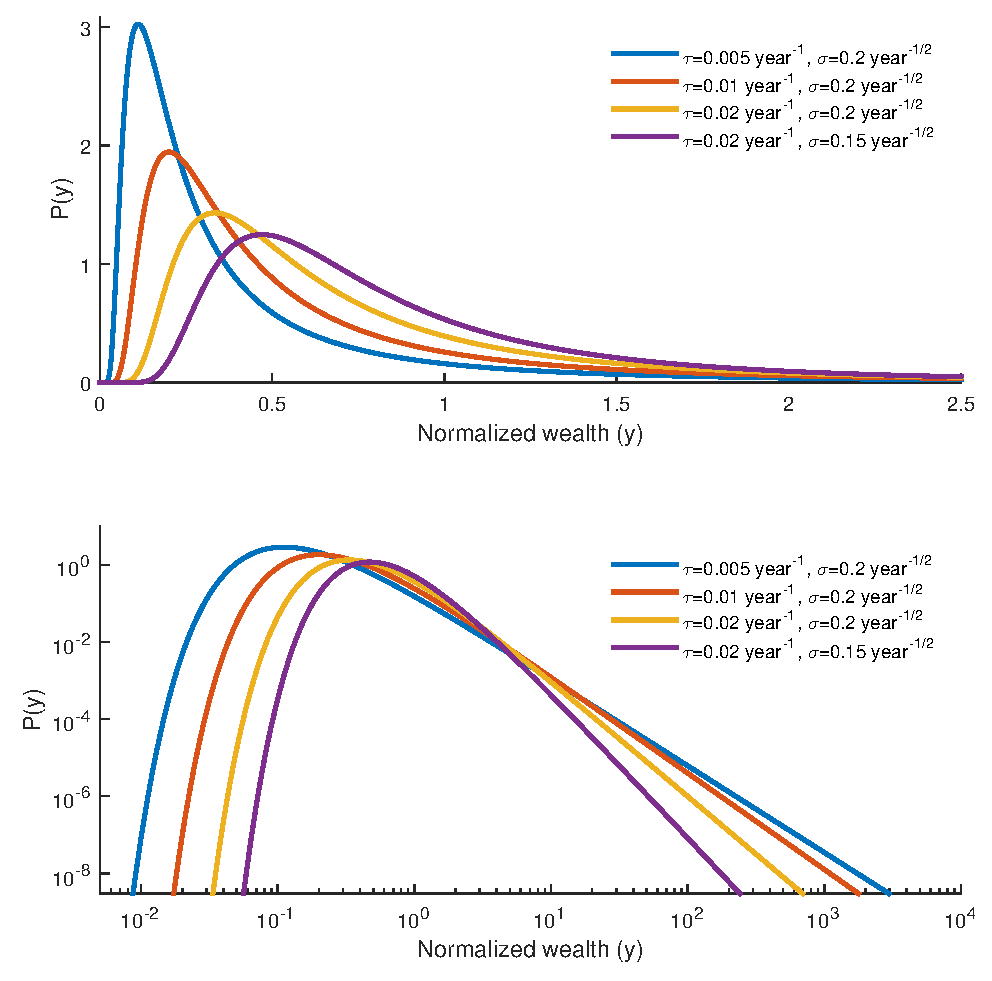
\includegraphics[width=1.0\textwidth] {./chapter_3/figs/dists.eps}
\caption{The stationary distribution for RGBM with positive $\tau$. Top -- linear scales; Bottom -- logarithmic scales.}
\flabel{dist}
\end{figure}

\paragraph{Negative $\tau$}

For $\tau<0$ the model exhibits mean repulsion rather than reversion. The ergodic hypothesis is invalid and no stationary wealth distribution exists. The population splits into those above the mean and those below the mean. Whereas in RGBM with non-negative $\tau$ it is impossible for wealth to become negative, negative $\tau$ leads to negative wealth. No longer is total economic wealth a limit to the wealth of the richest individual because the poorest develop large negative wealth. The wealth of the rich in the population increases exponentially away from the mean, and the wealth of the poor becomes negative and exponentially large in magnitude, see \Fref{regimes}. Qualitatively, this echoes the findings that the rich are experiencing higher growth rates of their wealth than the poor~\cite{Piketty2014,wolff2014household} and that the cumulative wealth of the poorest 50 percent of the American population was negative during 2008--2013~\cite{Rios20162013,WID2017}.

% AA comment on social mobility
Such splitting of the population is a common feature of non-ergodic processes. If rescaled wealth were an ergodic process, then individuals would, over long enough time, experience all parts of its distribution. People would spend 99 percent of their time as ``the 99 percent'' and 1 percent of their time as ``the 1 percent''. The social mobility that is, therefore, implicit in models that assume ergodicity might not exist in reality if that assumption is invalid. That inequality and immobility have been linked~\cite{Corak2013,LiuETAL2013,berman2017} may be unsurprising when both are viewed as consequences of non-ergodic wealth or income.

\begin{figure}[!htb]
\centering
\begin{tikzpicture}
%draw background
%\fill[draw=none, fill=lmlgrey, fill opacity=0.65] (0,0) rectangle (6,3);
%\fill[draw=none, fill=lmlgrey, fill opacity=0.25] (0,3) rectangle (6,6);

\fill[draw=none, pattern=north west lines, pattern color=black] (0,0.5) rectangle (5.9,3.5);
\fill[draw=none, pattern=crosshatch, pattern color=black] (0,3.5) rectangle (5.9,6.5);
\fill[draw=none, fill=white] (0.35,1) rectangle (5.55,3);
\fill[draw=none, fill=white] (0.35,4) rectangle (5.55,6);

%draw timeline
\draw [black,loosely dashed,ultra thick] (0,-0.5)--(0,0.5);
\draw[black,->,ultra thick,>=latex] (0,0.5)--(0,7.4) node[above left,rotate=90] {\small{ Reallocation rate ($\tau$)}};
  
% draw ticks
\draw [black,ultra thick] (-0.2,3.5)--(0.0,3.5);	\draw (-0.2,3.5) 	node[left=3pt] {\normalsize{$\scriptstyle 0$}};

%draw regime lines


%draw text

\node[black,font={\normalsize},anchor=west,text width=5cm] at (0.375,2.0) {No stationary distribution exists; wealths diverge -- some positive, some negative};
\node[black,font={\normalsize},anchor=west,text width=5cm] at (0.375,5.0) {Stationary distribution exists; some moments converge, some don't};
%\node[black,font={\footnotesize},anchor=west] at (0.1,1.3) {- No stationary distribution;};
%\node[black,font={\footnotesize},anchor=west] at (0.1,1.0) {- };
%\node[black,font={\footnotesize},anchor=west] at (0.1,0.7) {\,\, some negative};
%\node[black,font={\footnotesize},anchor=west] at (0.1,3.3) {- Stationary distribution exists;};
%\node[black,font={\footnotesize},anchor=west] at (0.1,3) {- Some moments converge,};
%\node[black,font={\footnotesize},anchor=west] at (0.1,2.7) {\,\, some don't};

%embed figs
\node[anchor=west] at (6,3.4)  {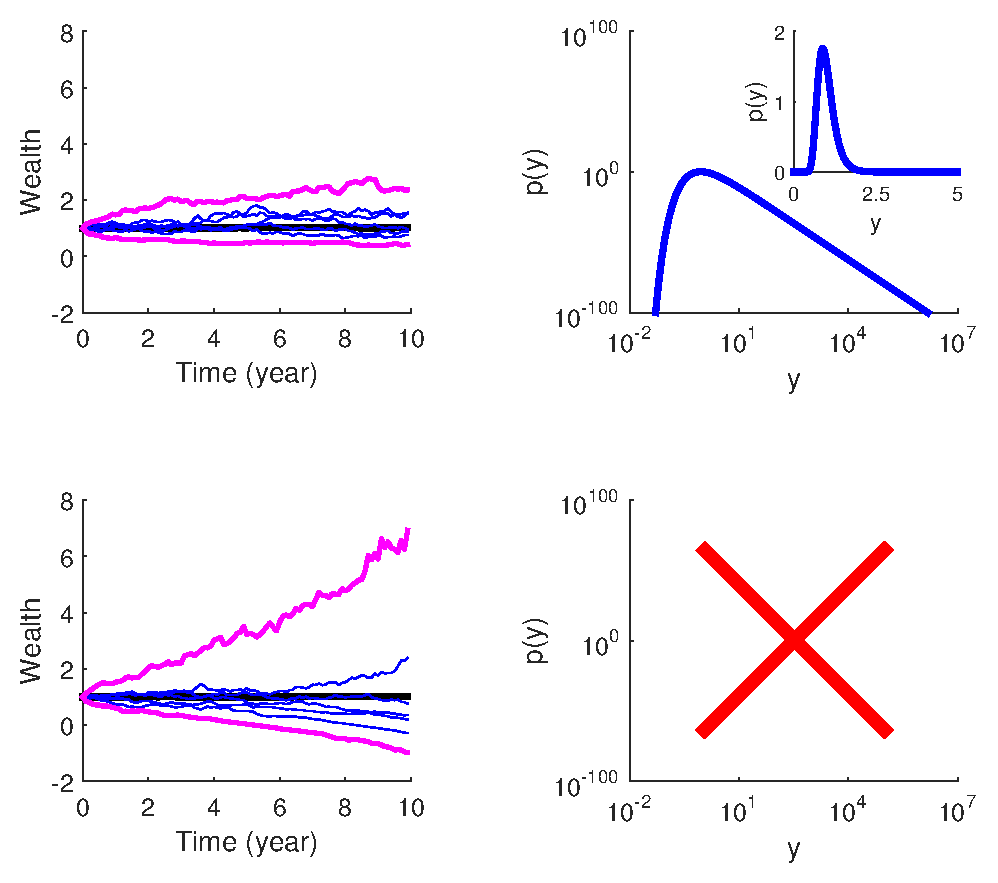
\includegraphics[height=6.5cm,keepaspectratio]{./chapter_3/figs/trajectories.eps}};
%\node[anchor=west] at (6,4.5)  {\includegraphics[height=3cm,keepaspectratio]{pos_tau1.eps}};
%\node[anchor=west] at (9.75,4.5)  {\includegraphics[height=3cm,keepaspectratio]{pos_tau3.eps}};
%\node[anchor=west] at (6,1.5)  {\includegraphics[height=3cm,keepaspectratio]{pos_tau2.eps}};

\draw [black,densely dashed,ultra thick] 			(0,3.5)--(13.5,3.5);

%labels
\node[black,font=\normalsize\sffamily,anchor=west,text width=4.5cm] at (0.2,6.75) {A)};
\node[black,font=\normalsize\sffamily,anchor=west,text width=4.5cm] at (5.85,6.75) {B)};
\node[black,font=\normalsize\sffamily,anchor=west,text width=4.5cm] at (9.7,6.75) {C)};
\node[black,font=\normalsize\sffamily,anchor=west,text width=4.5cm] at (5.85,3.15) {D)};
\node[black,font=\normalsize\sffamily,anchor=west,text width=4.5cm] at (9.7,3.15) {E)};
  
\end{tikzpicture}
\caption{Regimes of RGBM. A) $\tau=0$ separates the two regimes of RGBM. For $\tau>0$, a stationary wealth distribution exists. For $\tau<0$, no stationary wealth distribution exists and wealths diverge. B) Simulations of RGBM with $N=1000$, $\mu=0.021 \text{ year}^{-1}$ (presented after rescaling by $e^{\mu t}$), $\sigma=0.14\text{ year}^{-1/2}$, $x_i\left(0\right)=1$, $\tau=0.15 \text{ year}^{-1}$. Magenta lines: largest and smallest wealths, blue lines: five randomly chosen wealth trajectories, black line: sample mean. C) The stationary distribution to which the system in B) converges. Inset: same distribution on linear scales. D) Similar to B), with $\tau=-0.15 \text{ year}^{-1}$. E) in the $\tau<0$ regime, no stationary wealth distribution exists.}
\flabel{regimes}
\end{figure}

\section{Data}\label{sec:data}

\subsubsection{Wealth share data}

We analyze the wealth shares of the top quantiles of the US population, as estimated by three sources using different methods:

\bi
\item
The income tax method (``capitalization method'') that uses information on capital income from individual income tax returns to estimate the underlying stock of wealth~\cite{SaezZucman2014,WID2017}. ``If we can observe capital income $k = rW$, where $W$ is the underlying value of an asset and $r$ is the known rate of return, then we can estimate wealth based on capital income and capitalization factor $1/r$ defined using the appropriate choice of rate of return''~\cite[p.~54] {kopczuk2015we}. Data availability: the wealth shares of the top 5, 0.5, 0.1 and 0.01 percent for 1917--2012 and of the top 10 and 1 percent for 1913--2014 (annually).
\item
The estate multiplier method that uses data from estate tax returns to estimate wealth for the upper tail of the wealth distribution~\cite{kopczuk2004top}. ``The basic idea is to think of decedents as a sample from the living population. The individual-specific mortality rate $m_i$ becomes the sampling rate. If $m_i$ is known, the distribution for the living population can be simply estimated by reweighting the data for decedents by inverse sampling weights $1/m_i$, which are called `estate multipliers' ''~\cite[p.~53] {kopczuk2015we}. Data availability: the wealth shares of the top 1, 0.5, 0.25, 0.1, 0.05 and 0.01 percent for 1916--2000 (annually, with several missing years).
\item
The survey-based method that uses data from the Survey of Consumer Finances (SCF) conducted by the Federal Reserve, plus defined-benefit pension wealth, plus the wealth of the members of the Forbes 400~\cite{bricker2016measuring2}. Data availability: the wealth shares of the top 1 and 0.1 percent for 1989--2013 (for every three years).
\ei

These sources are based on different datasets and for different time periods. In the overlapping periods, they sometimes report markedly different wealth share estimates (see \Fref{data1}).

\begin{figure}[!htb]
\centering
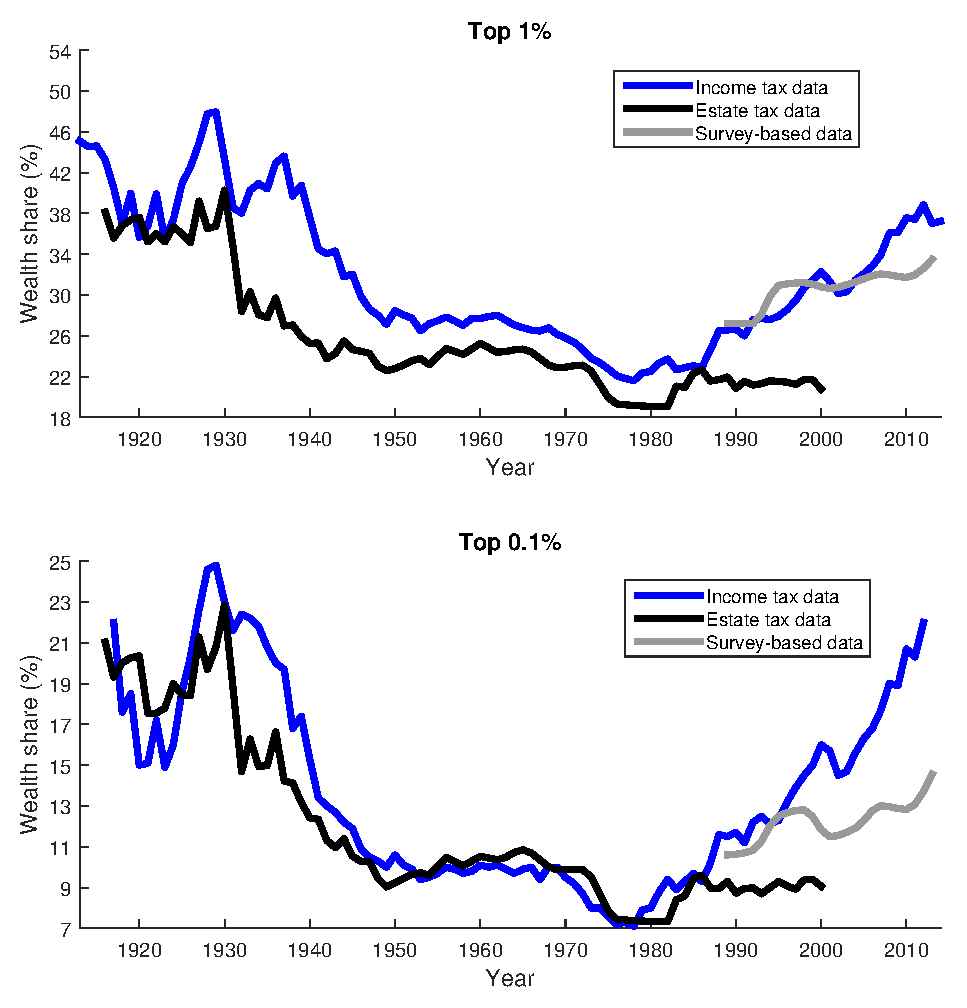
\includegraphics[width=1.0\textwidth] {./chapter_3/figs/data.eps}
\caption{The top wealth shares in the US, 1913--2014. Sources --~\cite{SaezZucman2014,WID2017} (blue);~\cite{kopczuk2004top} (black);~\cite{bricker2016measuring2} (grey).}
\flabel{data1}
\end{figure}

\cite{kopczuk2015we} reviewed the advantages and disadvantages of the different methods (see also the comment by Kopczuk on~\cite{bricker2016measuring2}). He observed that ``the survey-based and estate tax methods suggest that the share of wealth held by the top 1 percent has not increased much in recent decades, while the capitalization method suggests that it has''~\cite[p.~48] {kopczuk2015we}.

Which method best reflects the recent trends in wealth inequality is a matter of ongoing debate. Each method suffers from bias. For example, the survey-based method suffers from some underrepresentation of families who belong to the top end of the distribution. The income tax method suffers from some practical difficulties -- ``not all categories of assets generate capital income that appears on tax returns. [\ldots] Owner-occupied housing does not generate annual taxable capital income''~\cite[p. 54] {kopczuk2015we}. The estate tax method suffers from the need to accurately estimate mortality rates for the wealthy, known to be lower than those for the rest of the population. We refer the reader to~\cite{kopczuk2015we,bricker2016measuring2} for a thorough discussion. We analyze each data source separately.

%OP 20161108 updated up to here

\subsubsection{Wealth Growth Rate}
% AA20170120 - added new para and deleted old paras
We find numerically that the results of our analysis do not depend on $\mu$. This is because wealth shares depend only on the distribution of rescaled wealth and, for $\tau>0$, it is possible to scale out $\mu$ completely from the wealth dynamic to obtain \Eref{rgbm_ou_re} for rescaled wealth. The fitted $\tau<0$ values we find are not large or persistent enough to make our simulations significantly $\mu$-dependent. However, formally, since we allow negative $\tau$, we must simulate \Eref{rgbm} and not \Eref{rgbm_ou_re}. This requires us to specify a value of $\mu$, which we estimate as $\mu=0.021\pm 0.001 \text{ year}^{-1}$ by a least-squares fit of historical per-capita private wealth in the US~\cite{PikettyZucman2014} to an exponential growth curve.

%$\mu$, the exponential growth rate of individual wealth, is estimated from historical private wealth data for the US by dividing the total private wealth by the total population size~\cite{PikettyZucman2014}. In the analyzed data ``private wealth [...] is the net wealth (assets minus liabilities) of households and non-profit institutions serving households. [...] Assets include all the non-financial assets -- land, buildings, machines, and so on -- and financial assets, including life insurance and pensions funds, over which ownership rights can be enforced and that provide economic benefits to their owners''~\cite[p.~1268]{PikettyZucman2014}.
%
%Assuming the average historical private wealth grows exponentially, we found that $\mu=0.021\pm 0.001 \text{ year}^{-1}$ using a least-squares regression and this is the value used for our empirical analysis. 
%We note, however, that the wealth shares depend only on the distribution shape and not its mean. Therefore, our results are independent of $\mu$. We verified this numerically.

\subsubsection{Volatility}

% AA20170120 - edited to soften justification for using DJIA vol
We must also specify the volatility parameter, $\sigma$, in \Eref{rgbm}. In principle, this can vary with time. We have no access to real individual wealth trajectories, so we resort to estimating $\sigma\left(t\right)$ from other data. We find numerically that our results are not very sensitive to the details, so we need only a good ``ballpark'' estimate. We obtain that by assuming that the volatility in individual wealths tracks the volatility in the values of the companies that constitute the commercial and industrial base of the national economy. Therefore, for each year, we estimate $\sigma\left(t\right)$ as the standard deviation of daily logarithmic changes of the Dow Jones Industrial Average~\cite{Quandl2016}, which we annualise by multiplying by $\left(250/\text{year}\right)^{1/2}$. The values usually lie between $0.1$ and $0.2 \text{ year}^{-1/2}$, with an average of $0.16\text{ year}^{-1/2}$. Running our empirical analysis with constant $\sigma$ in this range had little effect on our results (see Appendix \ref{app:fixed_sig}) so, for simplicity, we present the analysis using $\sigma\left(t\right)=0.16\text{ year}^{-1/2}$ for all $t$.

Fitting $\sigma$ to stock market data means that we have only one model parameter -- the effective reallocation rate, $\tau\left(t\right)$ -- to fit to the historical wealth shares.

\subsubsection{Empirical Analysis}\label{sec:analysis}

The goal of the empirical analysis is to estimate $\tau\left(t\right)$ from the historical wealth data, using RGBM as our model. This estimation allows us to address two main questions:

\bi
\item[1.] Is it valid to assume ergodicity for the dynamics of relative wealth in the US? For the ergodic hypothesis to be valid, fitted values of $\tau\left(t\right)$ would have to be robustly positive.
\item[2.] If $\tau\left(t\right)$ is indeed positive, how long does it take for the distribution to converge to its asymptotic form?
\ei

%OP I rephrased this: any hint of non-positive $\tau$ means the ergodic hypothesis is a very bad idea.

We fit a time series, $\tau\left(t\right)$, that reproduces the annually observed wealth shares in the three datasets (see \secref{data}): Income tax-based~\cite{SaezZucman2014,WID2017}, estate tax-based~\cite{kopczuk2004top} and survey-based~\cite{bricker2016measuring2}. The wealth share, $S_q$, is defined as the proportion of total wealth, $\sum_i^N x_i$, owned by the richest fraction $q$ of the population, \eg $S_{10\%}=80 \text{ percent}$ means that the richest 10 percent of the population own 80 percent of the total wealth.

For an empirical wealth share time series, $S^{\text{data}}_q\left(t\right)$, we proceed as follows.

\bi
\item[ -- Step 1]
Initialise $N$ individual wealths, $\{x_i\left(t_0\right)\}$, as random variates of the inverse gamma distribution with parameters chosen to match $S^{\text{data}}_q\left(t_0\right)$.
\item[ -- Step 2]
Propagate $\{x_i\left(t\right)\}$ according to \Eref{rgbm} over $\Dt$,
%OP changed this: $\Dt$ is not always one year.
using the value of $\tau$ that minimises the difference between the wealth share in the modelled population, $S^{\text{model}}_q\left(t+\Dt, \tau\right)$, and $S^{\text{data}}_q\left(t+\Dt\right)$. We use the Nelder-Mead algorithm~\cite{NelderMead1965}.
\item[ -- Step 3]
Repeat Step 2 until the end of the time series.
\ei

We consider historical wealth shares of the richest $q=$ 10, 5, 1, 0.5, 0.25, 0.1, 0.05 and 0.01 percent and obtain time series of fitted effective reallocation rates, $\tau_q\left(t\right)$, shown in \Fref{tau}.
%\footnote{as described -- this fit is done separately for each quantile and for each dataset.}
%OP deleted footnote
For each value of $q$ we perform a run of the simulation for $N=10^8$. Since in practice $dW$ is randomly chosen, each run of the simulation will result in slightly different $\tau_q\left(t\right)$ values. However, we found that the differences between such calculations are negligible. 
%We observe a short spin-up period of approximately 2 years, after which $\tau_q\left(t\right)$ is no longer sensitive to the initial distribution.
%OP Deleted the comment about the spin-up period and sensitivity to initial distribution. We always use the inverse gamma dist. now so unclear what this sentence meant now.

\begin{figure}[!htb]
\centering
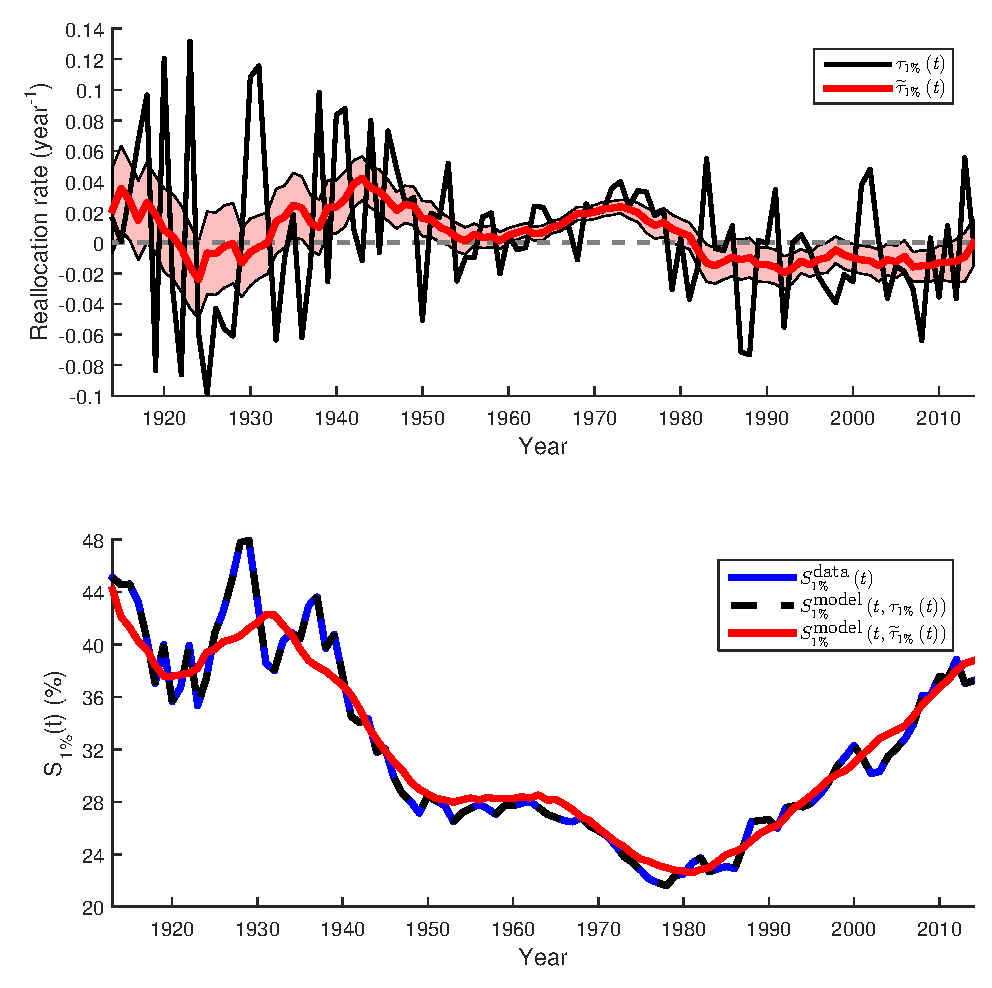
\includegraphics[width=1.0\textwidth] {./chapter_3/figs/tau_top1.eps}
\caption{Fitted effective reallocation rates. Calculations done using $\mu=0.021 \text{ year}^{-1}$ and $\sigma=0.16 \text{ year}^{-1/2}$. Top: $\tau_{1\%}\left(t\right)$ (black) and $\widetilde{\tau}_{1\%}\left(t\right)$ (red). Translucent envelopes indicate one standard error in the moving averages. Bottom: $S^{\text{data}}_{1\%}$ (blue), $S^{\text{model}}_{1\%}$ based on the annual $\tau_{1\%}\left(t\right)$ (dashed black), based on the 10-year moving average $\widetilde{\tau}_{1\%}\left(t\right)$ (red).}
\flabel{tau}
\end{figure}

\Fref{tau} (top) shows large annual fluctuations in $\tau_q\left(t\right)$. We are interested in longer-term changes in reallocation driven by structural economic and political changes. To elucidate these we smooth the data by taking a central 10-year moving average, $\widetilde{\tau}_q\left(t\right)$, where the window is truncated at the ends of the time series. To ensure the smoothing does not introduce artificial biases, we reverse the procedure and use $\widetilde{\tau}_q\left(t\right)$ to propagate the initially inverse gamma-distributed $\{x_i\left(t_0\right)\}$ and determine the wealth shares $S^{\text{model}}_q\left(t\right)$. The good agreement with $S^{\text{data}}_q\left(t\right)$ suggests that the smoothed $\widetilde{\tau}_q\left(t\right)$ is meaningful, see \Fref{tau} (bottom).

% AA20170120 - noted reallocation direction
For the income tax method wealth shares~\cite{SaezZucman2014}, the effective reallocation rate, $\widetilde{\tau}\left(t\right)$, has been negative -- \ie from poorer to richer -- since the mid-1980s. This holds for all of the inequality measures we derived from this dataset.

% AA20170120 - removed as this now repeats a similar para in the intro
%In a null model of a growing economy with social structure, data from the US economy in the last thirty years are best described by parameter values which imply net reallocation {\it from poorer to richer}. In other words, in spite of all the institutions society has built to redistribute resources from those with means to those without, net flows since the 1980s appear, in one dataset at least, to have been in the other direction.

For the survey-based wealth shares~\cite{bricker2016measuring2}, we observe briefer periods in which $\widetilde{\tau}\left(t\right) < 0$. The same is true for the estate tax data~\cite{kopczuk2004top}, see \Fref{shares_comp}. When $\tau\left(t\right)$ is positive, relevant convergence times are very long compared to the time scales of policy changes, namely at least several decades.

%It is not valid to assume ergodicity, and doing so can lead to severe misrepresentations of economic reality.
%OP: changed the above to avoid equivocating and confusing people.

All three datasets indicate that making the ergodic hypothesis is an unwarranted restriction on models and analyses. The hypothesis makes it impossible to observe and reason about the most dramatic qualitative features of wealth dynamics, such as rising inequality, negative reallocation, negative wealth, and social immobility.

\begin{figure}[!htb]
\centering
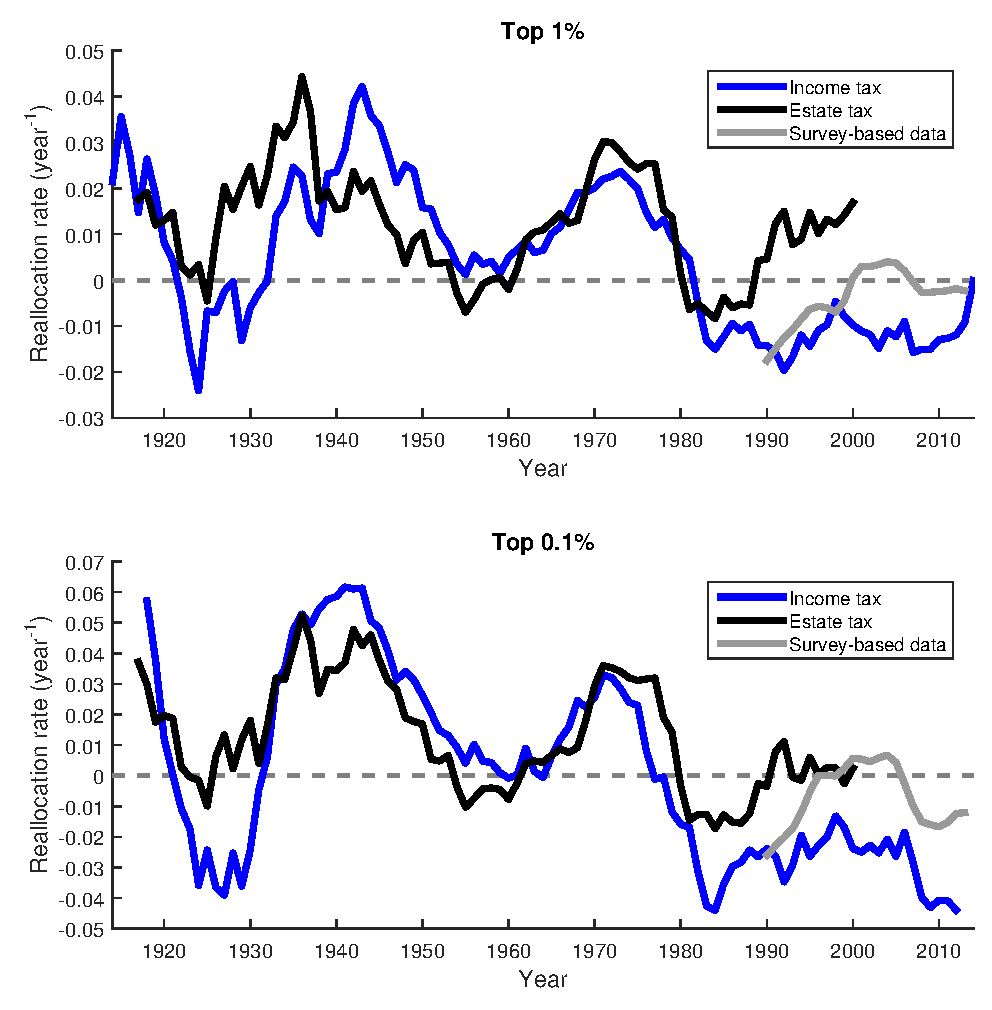
\includegraphics[width=1.0\textwidth] {./chapter_3/figs/tau_top1_top0i1_datasets.eps}
\caption{Effective reallocation rates for different datasets.}
\flabel{shares_comp}
\end{figure}

\subsubsection{Convergence times}

In the ergodic regime it is possible to calculate how fast the wealth shares of different quantiles converge to their asymptotic value. We do this numerically. Starting with a population of equal wealths and assuming $\mu=0.021 \text{ year}^{-1}$, $\sigma=0.16 \text{ year}^{-1/2}$, and $\tau = 0.04\text{ year}^{-1}$, we let the system equilibrate for 3000 years, long enough for the distribution to reach its asymptotic form to numerical precision. We then create a ``shock'', by changing $\tau$ to a different ``shock value'', and allow the system to equilibrate again for 3000 years, see top panel of \Fref{conv}. Following the shock, the wealth shares converge to their asymptotic values. We fit this convergence numerically with an exponential function and interpret the inverse of the exponential convergence rate as the convergence time. The bottom panel of \Fref{conv}  shows the convergence times versus the shock value of $\tau$.

\begin{figure}[!htb]
\centering
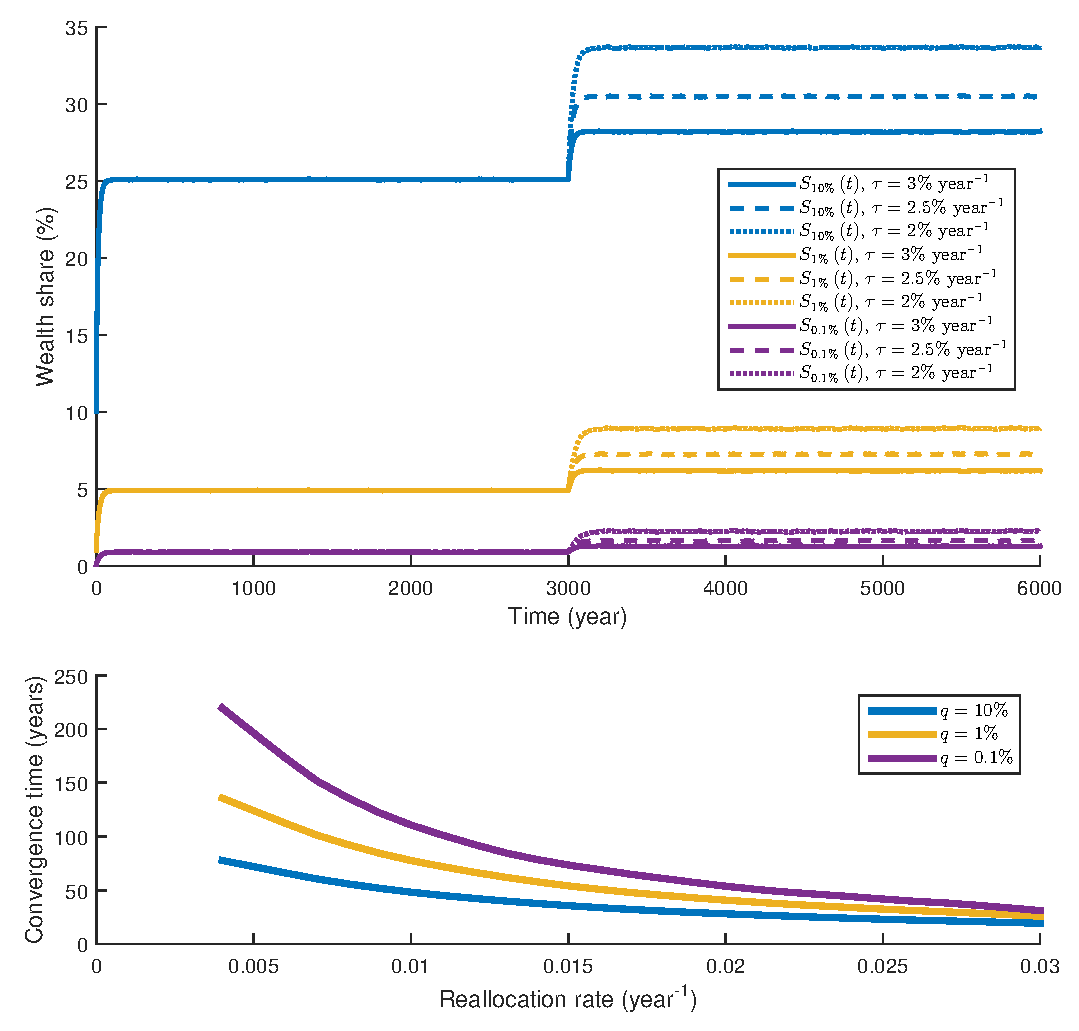
\includegraphics[width=1.0\textwidth] {./chapter_3/figs/convergence.eps}
\caption{Wealth share convergence time. Top: The convergence of the wealth share for $q=$ 10 percent (blue), $q=$ 1 percent (yellow) and $q=$ 0.1 percent (purple) following a change in the value of $\tau$ from $0.04\text{ year}^{-1}$ to $0.03\text{ year}^{-1}$ (solid), $0.025\text{ year}^{-1}$ (dashed) and $0.02\text{ year}^{-1}$ (dotted). Bottom: The wealth share exponential convergence time for $q=$ 10 percent (blue), $q=$ 1 percent (yellow) and $q=$ 0.1 percent (purple) as a function of $\tau$.}
\flabel{conv}
\end{figure}

In addition, it is possible to calculate the convergence time of the variance of the stationary distribution (and other cumulants and moments of interest). In the ergodic regime the stationary distribution has a finite variance only if $\tau > \sigma^2/2$~\cite{LiuSerota2016}. Convergence of the actual variance to the stationary variance occurs exponentially over a timescale $1/(2\tau - \sigma^2)$. \Fref{convar} shows the convergence times for different values of $\sigma$. See Appendix \ref{app:var_conv} for more details.

\begin{figure}[!htb]
\centering
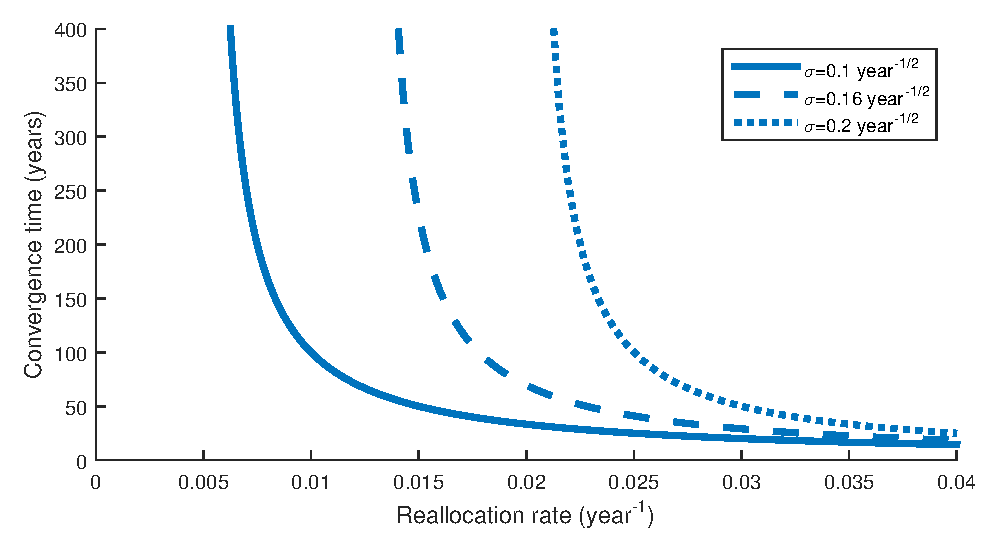
\includegraphics[width=1.0\textwidth] {./chapter_3/figs/variance_convergence.eps}
\caption{Variance convergence time}
\flabel{convar}
\end{figure}

%Convergence times for wealth shares and variance are long, ranging from a few decades to several centuries. Whether this is a practical problem depends on whether the  We arrive at this conclusion by assuming ergodicity in our model and observing far greater differences between model and reality than without the ergodic constraint. Specifically, we perform a different RGBM parameter fit, presented in \Fref{asymptau}. Here we find the reallocation rates, $\tau^\text{eqm}_q\left(t\right)$, that generate long-time stationary distributions consistent with observed wealth shares. In other words, we assume instantaneous equilibration. 

% AA edited above para. I found it difficult to parse, but also understood why changes were made. Below my best effort at merging old and new versions.
Convergence times for wealth shares and variance are long, ranging from a few decades to several centuries. This implies that empirical studies which assume ergodicity and fast convergence will be inconsistent with the data. To test this, we simulate such a study by performing a different RGBM parameter fit. We find the reallocation rates, $\tau^\text{eqm}_q\left(t\right)$, that generate stationary distributions consistent with observed wealth shares. In other words, we assume instantaneous convergence.

% AA20170120 -  moved before fig as fig no longer referenced in previous para
\Fref{asymptau} contrasts $\tau^\text{eqm}_{1\%}\left(t\right)$ assuming ergodicity with $\widetilde{\tau}_{1\%}\left(t\right)$ without assuming ergodicity (using the income tax method dataset). If convergence were always possible and fast, then the two values would be identical within statistical uncertainties. They are not. In addition, the generally large discrepancies between the wealth inequality implied by $\tau^\text{eqm}_{1\%}\left(t\right)$ (bottom panel, \Fref{asymptau}, green line) and as observed (bottom panel, \Fref{asymptau}, blue line) indicate that the wealth distribution does not stay close to its asymptotic form. This means that the long convergence times we calculate are a practical methodological problem for conventional studies.

\begin{figure}[!htb]
\centering
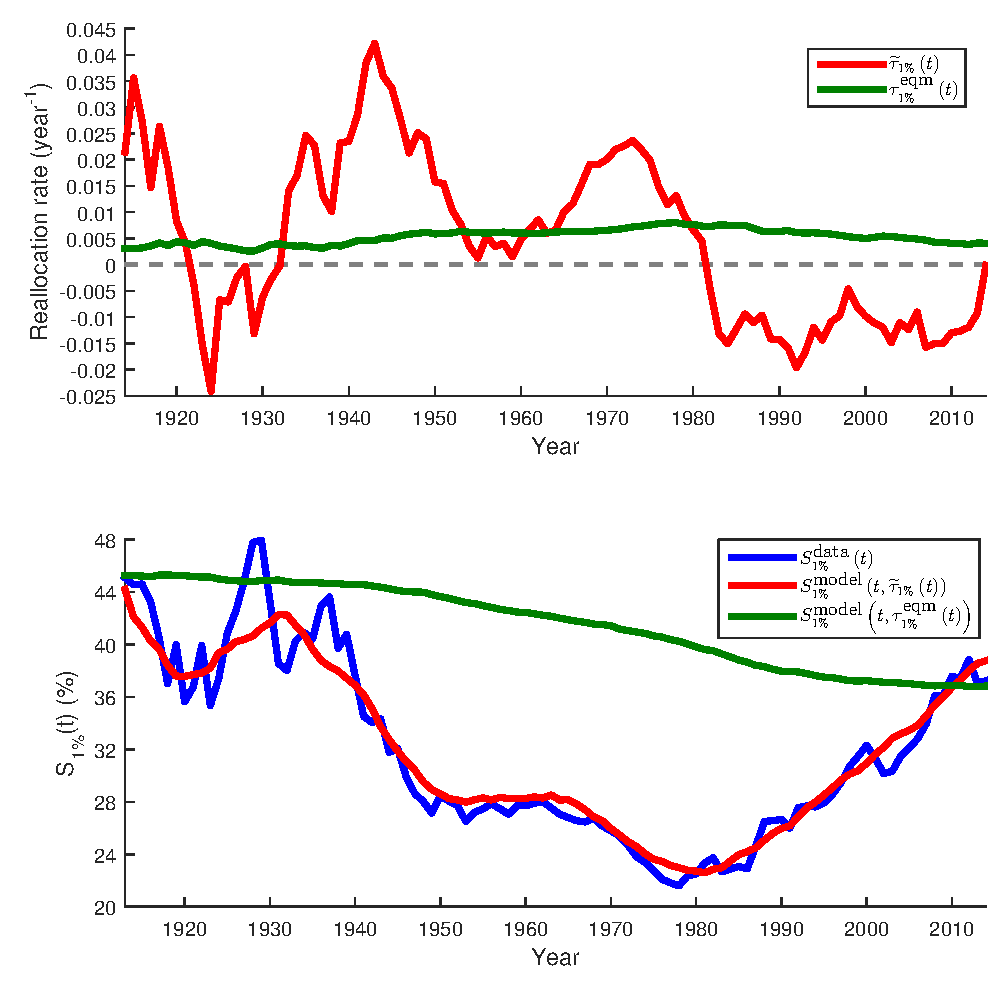
\includegraphics[width=1.0\textwidth] {./chapter_3/figs/tau_eqm_top1.eps}
\caption{Comparison of dynamic and equilibrium reallocation rates. Top: $\widetilde{\tau}_{1\%}\left(t\right)$ (red, same as in the top of \Fref{tau}). $\tau^\text{eqm}_{1\%}\left(t\right)$ (green), defined such that $\lim_{t'\to\infty} S^{\text{model}}_{1\%}\left(t',\tau^\text{eqm}_{1\%}\left(t\right)\right)=S^{\text{data}}_{1\%}\left(t\right)$. It is impossible by design for this value to be negative. The significant difference between the red and green lines demonstrates that the fast convergence assumption is invalid for the problem under consideration. Bottom: $S^{\text{data}}_{1\%}$ (blue), $S^{\text{model}}_{1\%}$ based on the 10-year moving average $\widetilde{\tau}_{1\%}\left(t\right)$ (red), based on $\tau^\text{eqm}_{1\%}\left(t\right)$ (green). The reallocation rates found under the fast convergence assumption generate model wealth shares which bear little relation to reality.}
\flabel{asymptau}
\end{figure}

\subsubsection{The effect of earnings}\label{sec:earnings}
% AA 20170516: Section edited to be more careful about phrases like ``in the absence of earnings''. Earnings are always present. The question is whether they are modelled explicitly or subsumed into the reallocation mechanism. 

In a recent review,~\cite[p.~593]{benhabib2017earnings} remark that ``the literature has largely emphasised the role of earnings inequality in explaining wealth inequality'' and point to empirical failures of this approach. The most popular models, in which agents accumulate wealth through stochastic earnings and precautionary savings, predict a positive correlation between earnings and wealth inequality, which is not observed in cross-country data, and struggle ``to reproduce the thick right tail of the wealth distribution observed in the data''~\cite[p.~593]{benhabib2017earnings}. The latter failure is also noted by~\cite{hubmer2016historical}.~\cite[p.~595]{benhabib2017earnings} conclude that ``other factors, like stochastic idiosyncratic returns on wealth'' must be at play.

Consistent with these observations, RGBM models wealth accumulation as a multiplicative process. Changes in individual wealth are composed of terms proportional to either individual wealth or average wealth, in effect generating stochastic idiosyncratic returns. Additive changes akin to labor income and consumption are not treated explicitly. Instead their effects are wrapped into the reallocation rate, $\tau$. While this parsimony makes the model tractable -- in that we can write down the rescaled wealth distribution, \Eref{disti}, for positive $\tau$ -- it makes it impossible to disentangle the various real-world drivers of the observed increase in wealth inequality. It is, therefore, legitimate to ask whether wealth is inherently unstable (because it is reallocated negatively) or whether the increase in wealth inequality is really due to changes in the earnings distribution. If the latter, then the negative reallocation found in RGBM would be an artefact of an underspecified model and an unreliable indicator that rescaled wealth is non-ergodic.

To ensure we are not fooling ourselves, we check this by adding to \Eref{rgbm} a term representing earnings, for which data are available. We find that earnings have had a small effect on the dynamics of the wealth distribution over the last century. Since about 2000 this may have contributed to the increase in wealth inequality, but in general the effect has been stabilizing.
% AA 20170616: The next sentence is problematic. When we write ``wealth by itself'' we really mean the counterfactual in which wealth evolves purely multiplicatively. In other words, it's a statement about the dynamics not about the observable. Edited for clarification.
% This implies that wealth by itself, \ie excluding any earnings, has been less stable than RGBM could lead one to believe
This implies that the purely multiplicative dynamics of wealth, \ie excluding additive earnings, have exhibited greater negative reallocation than fits to RGBM might suggest.

We separate earnings out as follows, in a model we call Earnings Geometric Brownian Motion (EGBM):
\be
dx_i=x_i \left[\left(\mu\left(t\right)-\tau^\text{EGBM}\left(t\right)\right)dt+\sigma\left(t\right) dW_i\left(t\right)\right]+ \ave{x}_N\tau^\text{EGBM}\left(t\right) dt + \epsilon_i\left(t\right) dt.
\elabel{egbm}
\ee
The notation is similar to RGBM, with the addition of the individual earnings term $\epsilon_i\left(t\right)$. We consider earnings after spending and after tax, as they directly change wealth. This changes the role of the reallocation rate, as reflected in the notation: $\tau^\text{EGBM}$ reflects changes in wealth for reasons other than additive income and consumption.

Using the same techniques as for the RGBM fits, we fit a time series, $\tau^\text{EGBM}\left(t\right)$, that reproduces annually observed wealth shares in the US (for the income tax method dataset). This requires us to find individual earnings in \Eref{egbm}, which we do as follows.
We assume that the earnings are log-normally distributed (see for example~\cite{pinkovskiy2009parametric}) and then fit the two parameters of the distribution every year. This is done using the mean earnings (calculated as total disposable national income multiplied by the personal savings rate and divided by the population size, as reported by~\cite{PikettyZucman2014}) and the top $1\%$ income share data (as reported in~\cite{WID2017}).

Since the joint wealth-earnings distribution is not known fully, we analyze two bounding scenarios. First, a ``correlated'' scenario in which earnings are perfectly correlated with wealth. Every year, the richest individual has the highest earnings, the second richest individual has the second highest earnings, and so on. This is the least stabilizing possibility. Second, an ``anti-correlated'' scenario in which the poorest individual has the highest earnings, the second poorest individual has the second highest earnings, and so on. This is the most stabilizing possibility. We fit $\tau^\text{EGBM}\left(t\right)$ for each scenario, and compare the results to the fitted $\tau\left(t\right)$ values for which the effects of earnings have not been disentangled from other effects. See \Fref{egbm}.

\begin{figure}[!htb]
\centering
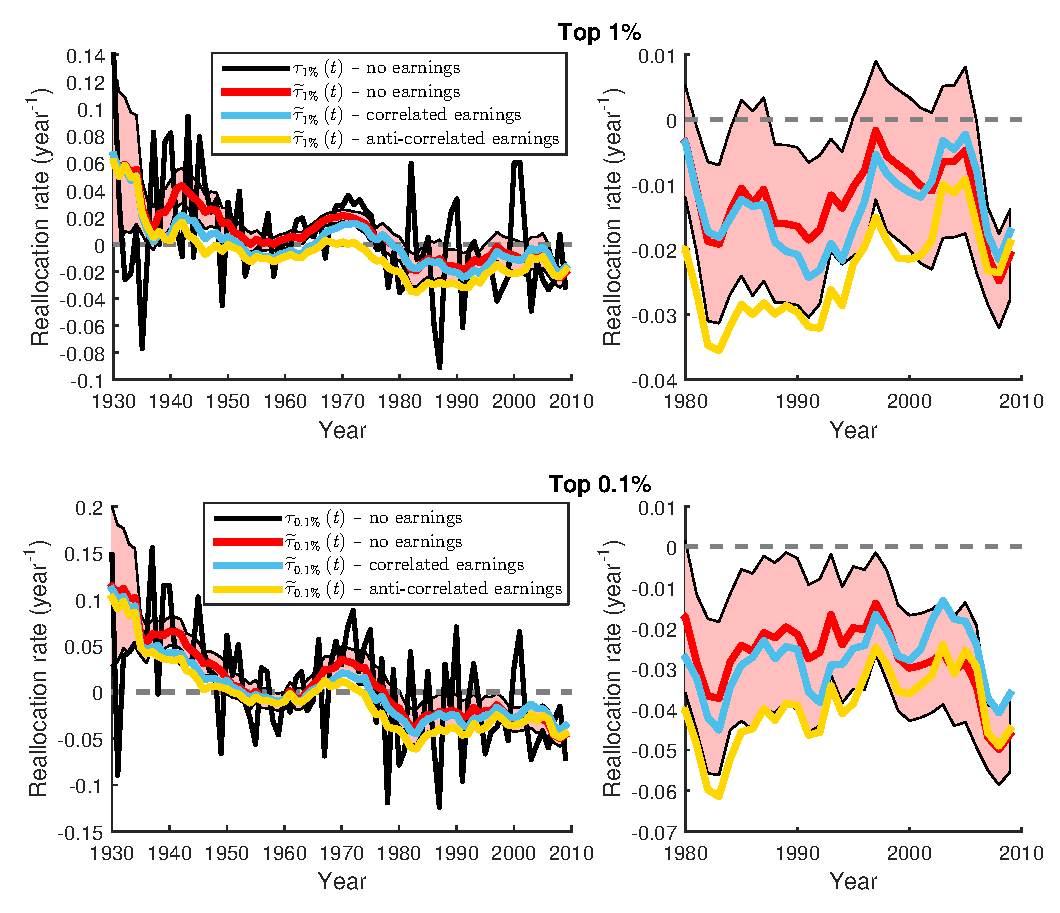
\includegraphics[width=1.0\textwidth] {./chapter_3/figs/tau_with_earnings.eps}
\caption{The effective reallocation rates for the RGBM and EGBM models. The red translucent envelopes indicate one standard error in the moving averages of the RGBM fitted reallocation rates.}
\flabel{egbm}
\end{figure}

In general, disentangling earnings has a small effect on the fitted reallocation rates. For the correlated scenario -- which is the more realistic of the two because the correlation between wealth and earnings is positive~\cite{Rios20162013} -- the fitted reallocation rates $\tau^\text{EGBM}\left(t\right)$ are within the statistical error of $\tau\left(t\right)$, into which the effects of earnings have been subsumed.

When earnings have a stabilizing effect, the fitted reallocation rate is lower under EGBM than under RGBM. Even in the correlated scenario, which is the least stabilizing, earnings have a stabilizing effect for years 1930--2000. During 2000--2010, we find that earnings destabilise the wealth distribution in the correlated scenario. However, since the difference between the fitted values is small, we can conclude that the contribution of earnings to the reported increase in wealth inequality from 1985 to 2010 is negligible. Moreover, the earnings contribution cannot explain the invalidity of the ergodic hypothesis that constitutes our main finding.

We suspect the main reason for the small effect of earnings is the low ratio of earnings to wealth. \Fref{ratio} shows the ratio of average earnings (after spending) to average wealth in the US during the period under study. Typically this ratio is around $1\%$, at which level earnings play only a secondary role in the dynamics of wealth. This echoes the observations of~\cite{Piketty2014,PikettyZucman2014,berman2017revisiting}. Under such conditions, it is unsurprising that models reliant on earnings as the primary mechanism of wealth accumulation fail to resemble reality~\cite{hubmer2016historical,benhabib2017earnings}. By including a multiplicative growth mechanism for wealth, RGBM avoids these pitfalls. Not only does it predict the Pareto tail of the stationary wealth distribution, when it exists, but also it allows for fitted tail exponents that reproduce the observed tail thickness (see \secref{model_behavior}). Retreating to the simplicity of RGBM is, therefore, justified.

\begin{figure}[!htb]
\centering
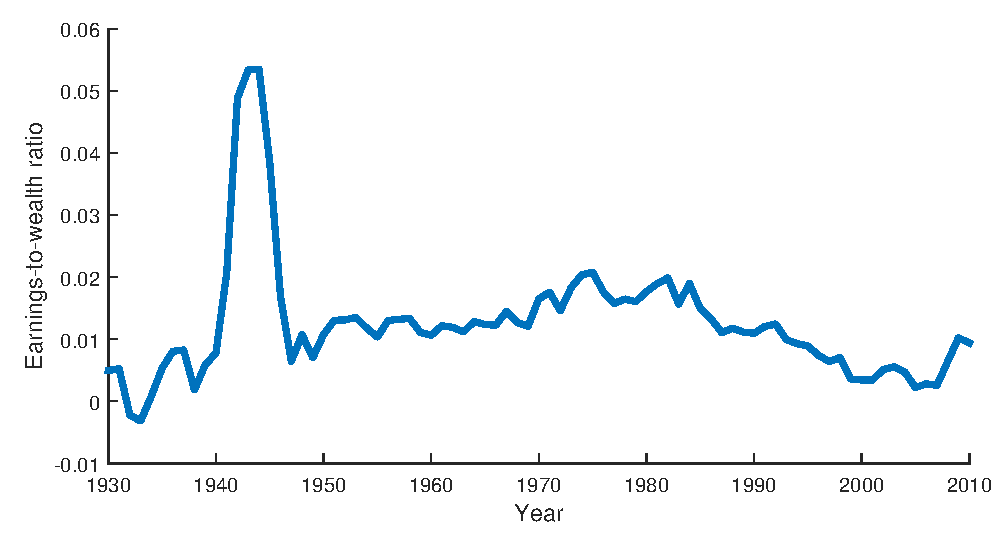
\includegraphics[width=1.0\textwidth] {./chapter_3/figs/earnings_to_wealth.eps}
\caption{Time series of the ratio of average earnings after spending to average private wealth in the US. Data from~\cite{PikettyZucman2014}.}
\flabel{ratio}
\end{figure}

\subsubsection{Conclusions}\label{sec:conclusions}

% AA20170120 - changed bullets to 1,2 to avoid confusion with A,B below
Studies of economic inequality often assume ergodicity of relative wealth. This assumption also goes under the headings of equilibrium, stationarity, or stability~\cite{AdamouPeters2016}. Specifically, it is assumed that:
\bi
\item[1.] the system can equilibrate, \ie a stationary distribution exists to which the observed distribution converges in the long-time limit; and
\item[2.] the system equilibrates quickly, \ie the observed distribution gets close to the stationary distribution after a time shorter than other relevant timescales, such as the time between policy changes.
\ei
Assumption 2 is often left unstated, but it is necessary for the stationary (model) distribution to resemble the observed (real) distribution. This matters because the stationary distribution is often a key object of study -- model parameters are found by fitting the stationary distribution to observed inequality, and effects of various model parameters on the stationary distribution are explored.

We do not assume ergodicity. Fitting $\tau$ in RGBM allows the data to speak without constraint as to whether the ergodic hypothesis is valid. We find it to be invalid because:
\bi
\item[A.] We observe negative $\tau$ values in all datasets analyzed, most notably using the income tax method, especially since about 1980. The wealth distribution is non-stationary and inequality increases for as long as these conditions prevail.
\item[B.] When we observe positive $\tau$, the associated convergence times are mostly of the order of decades or centuries, see \Fref{shares_comp} and \Fref{conv} (bottom). They are much longer than the periods over which economic conditions and policies change -- they are the timescales of history rather than of politics.
\ei
The ergodic hypothesis precludes what we find. Item A above corresponds to reallocation that moves wealth from poorer to richer individuals, which is inconsistent with the ergodic hypothesis. In this sense the ergodic hypothesis is a set of blindfolds, hiding from view the most dramatic economic conditions. For the most recent data, the system is in a state best described by non-ergodic RGBM, $\tau<0$~\cite{SaezZucman2014,WID2017} or $\tau \approx 0$~\cite{bricker2016measuring2}. Therefore, each time we observe the wealth distribution, we see a snapshot of it either in the process of diverging or very far from its asymptotic form. It is much like a photograph of an explosion in space: it will show a fireball whose finite extent tells us nothing of the eventual distance between pieces of debris.

We also find that changes in the earnings distribution do not provide an adequate alternative explanation of the described dynamics of the wealth distribution. Although earnings have become more unequal over the recent decades in which wealth inequality has increased, their effect on the wealth distribution has been small and generally stabilizing rather than destabilizing. Treating earnings explicitly in our model does not change fundamentally our conclusions.

The economic phenomena that trouble theorists most -- such as diverging inequality, social immobility, and the emergence of negative wealth -- are difficult to reproduce in a model that assumes ergodicity. In our simple model, this is easy to see: in the ergodic regime, $\tau>0$, our model cannot reproduce these phenomena at all. One may be tempted to conclude that their existence is a sign of special conditions prevailing in the real world -- collusion and conspiracies. But if we admit the possibility of non-ergodicity, $\tau\leq0$, it becomes clear that these phenomena can easily emerge in an economy that does not actively guard against them.

\subsubsection{The derivation of self-averaging time $t_c$}\label{app:tauc}

In transforming the differential equation for wealth, $x$, into a differential equation for rescaled wealth, $y$, we use the approximation $\ave{x\left(t\right)}_N=\ave{x\left(0\right)}_N e^{\mu t}$. In other words we assume that the population-average wealth grows like the expectation value of wealth. 

It is known that this approximation is invalid for long times~\cite{PetersKlein2013}. Specifically, over long times $\ave{x\left(t\right)}_N$ grows at the exponential rate $\mu-\sigma^2/2$, whereas the expectation value, $\ave{x\left(t\right)}$, grows at the exponential rate $\mu$.

This raises the question for how long our approximation is valid. 
The answer depends on the sample size $N$, as it must because the expectation value is just the $N\to\infty$ limit of the population average.
To assess whether the fluctuations in $\ave{x\left(t\right)}_N$ are important, we compare the variance of $\ave{x\left(t\right)}_N$ to the expectation value squared (equivalent to comparing the standard deviation to the expectation value). 
If the variance is smaller than the expectation value squared, then the approximation is acceptable. 
If this is not the case, then we cannot use this approximation.

The calculations that use the approximation relate to properties of the stationary distribution. This exists for $\tau$ above some positive threshold, \ie with sufficiently strong reallocation. The coupling of wealth trajectories through reallocation lengthens the timescale over which the population average resembles the expected wealth. Therefore, we are on safe ground if we can show that the timescale on which the approximation is valid when $\tau=0$ is longer than practically relevant timescales. This is a sufficient condition for the approximation to be valid when $\tau>0$.

This means we work with a population of $N$ independent GBMs, which makes the computation of the variance easy. GBM is log-normally distributed,
\be
\ln\left[x\left(t\right)\right]\sim \ln\mathcal{N}\ln\left(x\left(0\right)+\left[\mu-\frac{\sigma^2}{2}\right] t, \sigma^2 t\right).
\ee
From this, it follows that the expectation value of a single trajectory grows as
\be
\ave{x\left(t\right)}=x\left(0\right)e^{\mu t},
\ee
and the variance grows as
\be
V\left[x\left(t\right)\right]=x\left(0\right)^2 e^{2\mu t}\left[e^{\sigma^2 t}-1\right].
\ee

Because the wealth trajectories are independent, the variance of an average over $N$ trajectories is one-$N^{\text{th}}$ of the variance for the individual trajectory.  
We are now in a position to compare standard deviation and average as follows
\be
\frac{V\left[\ave{x\left(t\right)}_N\right]}{\ave{\ave{x\left(t\right)}_N}^2} = \frac{e^{\sigma^2 t}-1}{N}\,.
\ee
So long as this is less than one, $\ave{x\left(t\right)}$ is a good approximation for $\ave{x\left(t\right)}_N$. Rearranging and taking $N\gg1$ gives an upper bound on the time for which this approximation holds:
\be
t < t_c \equiv \frac{\ln N}{\sigma^2}.
\ee

For typical parameter values in our model, $N=10^8$ and $\sigma=0.16\, \text{year}^{-1/2}$, we find $t_c\approx 700$ years. It turns out that, strictly speaking, the minimum value of $\tau$ required for the stationary distribution to exist is not zero but proportional to the inverse of this timescale~\cite{Bouchaud2015b}, \ie 
\be
\tau > \tau_c \equiv \frac{\sigma^2}{2\ln N}.
\elabel{tauc}
\ee
In essence, the inequality-increasing effects of multiplicative growth drive wealths apart on the timescale $t_c$, whereas the inequality-reducing effects of reallocation drive wealths back together on the timescale $1/\tau$. Thus, $\tau_c$ marks the point at which reallocation overcomes the forces that drive wealths apart, leading to a stationary distribution of rescaled wealth. In our case $\tau_c\approx 0.0007 \text{ year}^{-1}$, which is in practice indistinguishable from zero.

The timescale $t_c$ was derived assuming that everyone starts out equally, which is not generally the case. If the initial distribution of wealth is very unequal, then the variance of $\ave{x}_N$ will be dominated by the fluctuations experienced by the wealthiest individuals, and the approximation $\ave{x}_N\approx \ave{x\left(0\right)}_N e^{\mu t}$ becomes invalid more quickly. We confirmed numerically that the effect is negligible for our study: our results are indistiguishable whether we simulate $dx$ (which requires an estimate for $\mu$), or $dy$ (where $\mu$ does not appear but the above-mentioned approximation is made).

\clearpage

\subsubsection{The derivation of the stationary distribution}\label{app:stat}

We start again with the SDE for the rescaled wealth, 
\be
dy= \sigma\,y\,dW - \tau\left(y - 1\right)dt.
\ee
This is an It\^o equation with drift term 
$A=\tau(y - 1)$ and diffusion term $B=y \sigma$.

Such equations imply ordinary second-order differential equations that describe the evolution of the pdf, called Fokker-Planck equations. 
The Fokker-Planck equation describes the change in probability density, at any point in (relative-wealth) space, due to the action of the drift term (like advection in a fluid) and due to the diffusion term (like heat spreading). In this case, we have
\be
\frac{dp\left(y,t\right)}{dt}=\frac{\partial}{\partial y} \left[Ap\left(y,t\right)\right]+\frac{1}{2} \frac{\partial^2}{\partial y^2}\left[B^2 p\left(y,t\right)\right].
\ee

The steady-state Fokker-Planck equation for the pdf $p\left(y\right)$ is obtained by setting the time derivative to zero,
\be
\frac{\sigma^2}{2}\left(y^2 p\right)_{yy} + \tau\left[\left(y-1\right)p\right]_y = 0.
\elabel{fokker_planck}
\ee
Positive wealth subjected to continuous-time multiplicative dynamics with non-negative reallocation can never reach zero. Therefore, we solve \Eref{fokker_planck} with boundary condition $p\left(0\right)=0$ to give
\be
p\left(y\right) = C\left(\zeta\right) e^{-\frac{\zeta-1}{y}}y^{-\left(1+\zeta\right)}\,,
\ee
where 
\be
\zeta = 1+\frac{2\tau}{\sigma^2}
\ee
and
\be
C\left(\zeta\right) = \frac{\left(\zeta -1\right)^\zeta}{\Gamma \left(\zeta \right)}\,,
\ee
with the gamma function $\Gamma\left(\zeta\right) = \int_0^\infty x^{\zeta-1} e^{-x}\,\mathrm{d}x$. The distribution has a power-law tail as $y\to\infty$, resembling Pareto's often confirmed observation that the frequency of large wealths tends to decay as a power law. The exponent of the power law, $\zeta$, is called the Pareto parameter and is one measure of economic inequality.

\clearpage

\subsubsection{The effect of fixed versus time-varying $\sigma$}\label{app:fixed_sig}

Our analysis requires us to set the volatility parameter, $\sigma$, in the RGBM model. We estimate this as a time-varying quantity, $\sigma \left(t\right)$, using data from the American stock market. For each year in the analysis, we define $\sigma \left(t\right)$ as the standard deviation of the daily logarithmic changes in the Dow Jones Industrial Average (DJIA) for that year~\cite{Quandl2016}, annualised by multiplying by $\left(250/\text{year}\right)^{1/2}$. We present this in \Fref{sigmat}.

\begin{figure}[!htb]
\centering
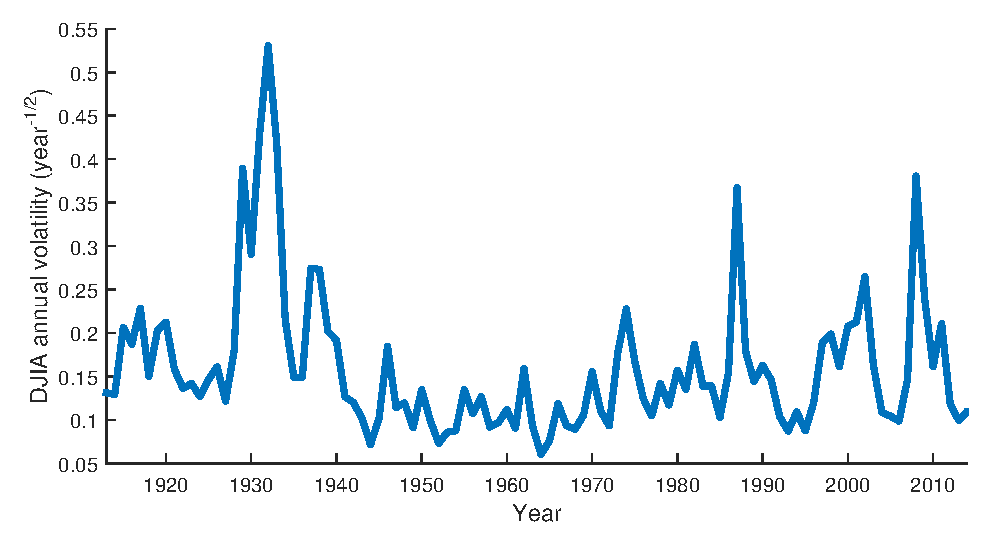
\includegraphics[width=1.0\textwidth] {./chapter_3/figs/DOW.eps}
\caption{Annualised $\sigma\left(t\right)$ estimated from daily changes in the DJIA. Data taken from~\cite{Quandl2016}.}
\flabel{sigmat}
\end{figure}

In the results presented in \secref{analysis}, we used a fixed value -- $\sigma=0.16$, the average of the time-varying $\sigma \left(t\right)$ -- for simplicity. In order to show this has little effect on the estimated reallocation rates, a comparison is presented in \Fref{sigmat_tau}.

\begin{figure}[!htb]
\centering
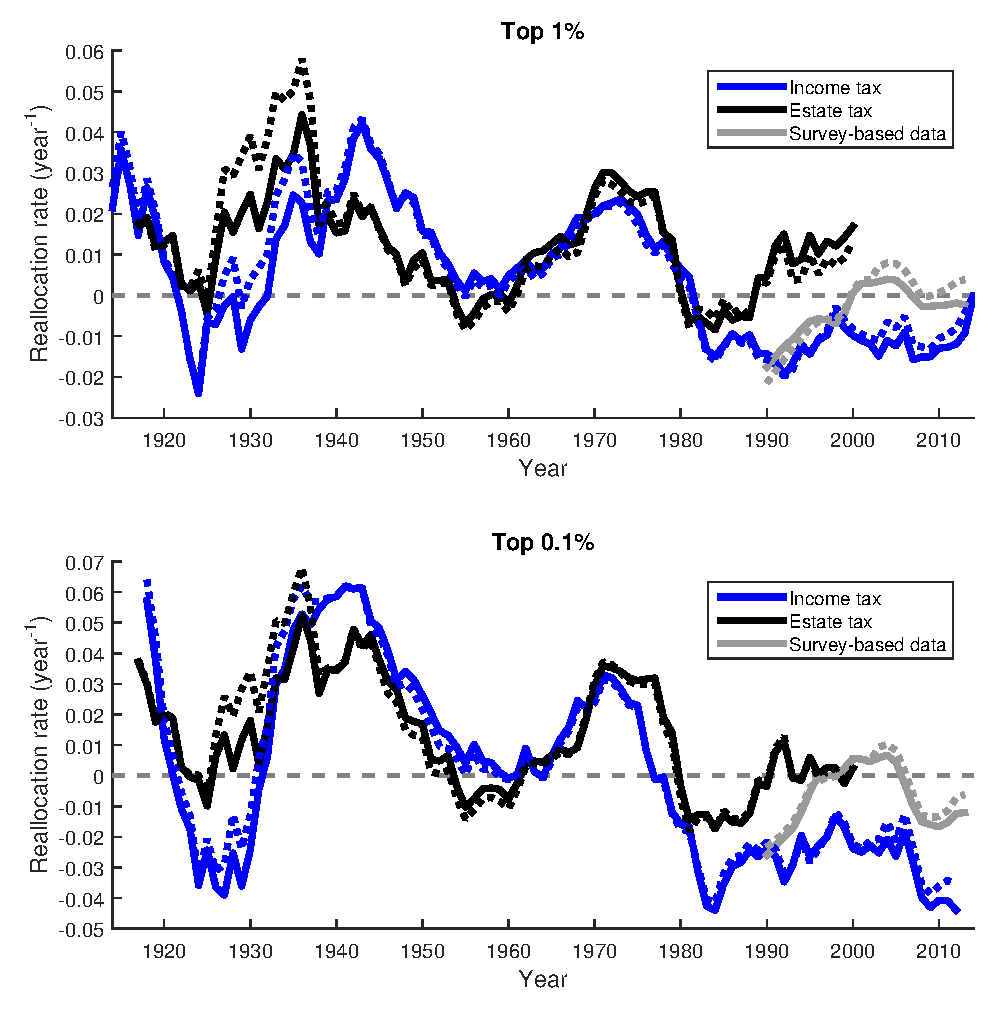
\includegraphics[width=1.0\textwidth] {./chapter_3/figs/sigma_fixed_notfixed_1_0i1.eps}
\caption{Smoothed effective reallocation rates with fixed and time-varying $\sigma$. Solid lines -- fixed $\sigma$; Dotted lines -- time-varying $\sigma$.}
\flabel{sigmat_tau}
\end{figure}

\clearpage

\subsubsection{The derivation of the variance convergence time}\label{app:var_conv}

Our key finding is that under currently prevailing economic conditions it is not safe to assume the existence of stationary wealth distributions in models of wealth dynamics. 
Nevertheless, we present some results for the regime of our model where a stationary distribution exists.
The full form of the distribution is derived in Appendix \ref{app:stat}. Because it has a power-law tail for large wealths, only the lower moments of the distribution exist, while higher moments diverge.
Below, we derive a condition for the convergence of the variance and calculate its convergence time.

The variance of $y$ is a combination of the first moment, $\ave{y}$ (the average), and the second moment, $\ave{y^2}$:
\be
V\left(y\right)=\ave{y^2}-\ave{y}^2
\ee
We thus need to find $\ave{y}$ and $\ave{y^2}$ in order to determine the variance. 
The first moment of the rescaled wealth is, by definition, $\ave{y}=1$. 

To find the second moment, we start with the SDE for the rescaled wealth:
\be
dy = \sigma y\,dW - \tau\left(y - 1\right)\,dt.
\elabel{rescaledSDE}
\ee

This is an It\^o process, which implies that an increment, $df$, in some (twice-differentiable) function $f\left(y,t\right)$ will also be an It\^o process, and such increments can be found by Taylor-expanding to second order in $dy$ as follows:
\be
df = \frac{\partial f}{\partial t} dt + \frac{\partial f}{\partial y} dy + \frac{1}{2}\frac{\partial^2 f}{\partial y^2} dy^2\,.
\ee
We insert $f\left(y,t\right)=y^2$ and obtain
\be
d \left(y^2\right) = 2ydy + \left(dy\right)^2\,.
\elabel{diff2}
\ee

We substitute $dy$ in \Eref{diff2}, which yields terms of order $dW$, $dt$, $dW^2$, $dt^2$, and $\left(dW\,dt\right)$. The scaling of Brownian motion allows us to replace $dW^2$ by $dt$, and we ignore $o\left(dt\right)$ terms. This yields
\bea
d \left(y^2\right) = 2\sigma y^2\,dW - \left(2\tau-\sigma^2\right) y^2\,dt + 2\tau y\,dt %+ \tau^2\left(y - 1\right)^2\,dt^2 - \st{\tau\left(y - 1\right)\,\sigma y\,dW\,dt}
\eea
Taking expectations on both sides, and using $\ave{y}=1$, produces an ordinary differential equation for the second moment:
\be
\frac{d \langle y^2 \rangle}{dt} = -\left(2\tau - \sigma^2\right) \langle y^2 \rangle + 2\tau
\elabel{avediff2}
\ee
with solution
\be
\langle y\left(t\right)^2 \rangle = \frac{2\tau}{2\tau - \sigma^2} + \left(\langle y\left(0\right)^2 \rangle - \frac{2\tau}{2\tau - \sigma^2}\right) e^{-\left(2\tau - \sigma^2\right)t}\,.
\elabel{avediff3}
\ee

The variance $V\left(t\right)=\langle y\left(t\right)^2 \rangle-1$ therefore follows
\be
V\left(t\right) = V_{\infty}+\left(V_0 - V_{\infty}\right)e^{-\left(2\tau - \sigma^2\right)t}\,,
\elabel{var1}
\ee
where $V_0$ is the initial variance and
\be
V_{\infty} = \frac{2\tau}{2\tau - \sigma^2}\,.
\elabel{varinf}
\ee
$V$ converges in time to the asymptote, $V_{\infty}$, provided the exponential in \Eref{var1} is decaying. 
This can be expressed as a condition on $\tau$
\be
\tau > \frac{\sigma^2}{2} \,.
\ee

Clearly, for negative values of $\tau$ the condition cannot be satisfied, and the variance (and inequality) of the wealth distribution will diverge. 
In the regime where the variance exists, $\tau > \sigma^2/2$, it also follows from \Eref{var1} that the convergence time of the variance is $1/\left(2\tau - \sigma^2\right)$.

As $\tau$ increases, increasingly high moments of the distribution become convergent to some finite value. 
The above procedure for finding the second moment (and thereby the variance) can be applied to the $k^\text{th}$ moment, just by changing the second power $y^2$ to $y^k$, and any other cumulant can therefore be found as a combination of the relevant moments. 
For instance~\cite{LiuSerota2016} also compute the third cumulant.


\subsection{\seclabel{Taxation}Taxation}
In \secref{Every_man} we created a world of independent GBMs; in \secref{Cooperation} 
we introduced to this world
the invention of cooperation and saw that it increases long-time growth for those who participate
in resource-pooling and sharing. In this section we study what happens if a large number
of individuals pool and share a small fraction of their resources, which is reminiscent of taxation
and redistribution carried out in a large population. We will find that while cooperation for 2 individuals
increases their growth rates, sufficient cooperation in a large population
has two related effects. Firstly, everyone's wealth grows asymptotically at a rate close to that of
the expectation value. Secondly, wealth condensation and the divergence of inequality 
no longer occur.

We introduce a model that applies a flat wealth tax rate and every individual, irrespective of his 
wealth, receives the same benefit from the collected tax, in absolute terms. This mimicks the
actions of a central agency that collects each year from everyone 1\% of his wealth and pays 
1-$N^\text{th}$ of the total collected amount to each individual. A similar model will be 
used for income tax, see \eref{isde} in \secref{Income_tax}. 

Of course this isn't how taxation works in reality -- wealth taxes are usually only collected in 
the form of inheritance tax and sometimes property or land tax; often progressive rates are 
applied, and how tax takings are actually redistributed is very unclear. 
Who benefits from government activity? Infrastructure is built, benefits payments made, 
healthcare and education provided, a legal system is maintained of courts that can 
enforce contracts and enable corporate structures, police and an army may provide security. 
Individuals will benefit from these different aspects to very different degrees. Our model 
ignores this and lets everyone benefit equally.

Despite the simplicity of the setup the following important feature emerges:
there is a critical tax rate. This qualitative result applies both to income tax and to wealth tax.

\definition{ {\bf Critical tax rate}\\
Below the critical tax rate the variance of rescaled wealth increases indefinitely. 
Above the critical tax rate it stabilizes to an asymptotic value in the limit $t\to\infty$.
}

\Secref{Cooperation} was concerned with growth, here we are concerned with inequality. 
We will therefore work with the rescaled wealth, $y$, introduced in \eref{rescaled}. \Eref{GBM} defines the 
dynamic of $x$. From it we can find the dynamic for $f(x)=y$ using \Ito calculus
\bea
df &=& \frac{\partial f}{\partial x} dx + \frac{\partial f}{\partial t} + \frac{1}{2} \frac{\partial^2 f}{\partial x^2} dx^2\\
=dy&=& -\mu y dt + \frac{y}{x} dx\\
&=&y \sigma dW.
\eea



\subsubsection{Wealth tax}
\seclabel{Wealth_tax}
We investigate the situation where each individual's wealth is taxed at a rate of $0\leq\tau\leq1$ per unit time, 
and the total tax thus raised is redistributed equally among the population. This is modelled by the stochastic wealth process,
\be
dx = x[(\mu-\tau)\,dt + \sigma\,dW] + \tau\ave{x}_N dt,
\elabel{wsde}
\ee
which is a modified version of \eref{GBM} -- the term $-\tau x dt$ was added to represent tax 
collection, and the term $+\tau \ave{x}_N dt$ to represent redistribution of collected tax.
To make the model more tractable we consider the case $N \to \infty$, which replaces the finite-ensemble 
average by the expectation value, $\ave{x}_N \to \ave{x}$. The finite ensemble size has important effects but 
we will not discuss them here.
Total wealth is conserved by the taxation and redistribution process in this model, 
and the expectation value is unaffected, $\ave{x(t)}=\ave{x_0}e^{\mu t}$, just as for GBM without taxation, \eref{exp_x}. 
We are again interested in rescaled wealth, $y=\frac{x}{\ave{x}}=x e^{-\mu t}$ (\eref{rescaled}), whose dynamic we derive using the chain rule
\bea
dy &=& \frac{\partial y}{\partial t}\,dt + \frac{\partial y}{\partial x}\,dx + \frac{1}{2} \frac{\partial^2 y}{\partial x^2} \,dx^2 \\
&=& -\mu y\,dt + \frac{1}{x}\,dx \elabel{ysde} \\
&=& y(-\tau dt+ \sigma dW)+\tau dt.
\eea
The first moment of $y$ is trivially $1$,
\be
\ave{y}=\ave{\frac{x}{\ave{x}}}=1.
\ee
We compute the dynamic of the second moment of $y$, to first order in $dt$, using the chain rule again,
\bea
d(y^2)&=& \frac{\partial (y^2)}{\partial t}\,dt + \frac{\partial (y^2)}{\partial y}\,dy + \frac{1}{2} \frac{\partial^2 (y^2)}{\partial y^2} \,(dy)^2\\
&=&2y dy + (dy)^2\\
&=& 2y^2(-\tau dt+ \sigma dW)+2y\tau dt +y^2\sigma^2 dt.
\eea
Taking expectation values yields 
\bea
\ave{dy^2}&=& \ave{-2y^2(-\tau dt+ \sigma dW)+2y\tau dt -y^2\sigma^2dt}\\
=d\ave{y^2}&=&(\sigma^2-2\tau) \ave{y^2} dt + 2\tau dt.
\eea
This equation is an inhomogeneous first-order ordinary differential equation for 
the second moment. Perhaps it's more recognizable when written in standard form as
\be
\left(\frac{d}{dt}- (\sigma^2-2\tau)\right)\ave{y^2}= 2\tau.
\elabel{ODE2}
\ee
Such equations are solvable using the method of integrating factors, see \eg \cite[Chpater 1.5]{BenderOrszag1978}.
The solution of the dynamic \eref{ODE2} is the second moment 
of the distribution of rescaled wealth as a function of time, namely
\be
\ave{y^2} = \frac{2\tau}{2\tau-\sigma^2} + \left(\ave{y_0^2} - \frac{2\tau}{2\tau-\sigma^2}\right) e^{-(2\tau-\sigma^2)t}.
\ee
This can be rewritten in terms of the variance of rescaled wealth, $V=\ave{y^2}-1$, as
\be
V(t) = V_\infty + (V_0 - V_\infty) e^{-(2\tau-\sigma^2)t},
\elabel{wvar}
\ee
where $V_0$ is the initial variance and
\be
V_\infty \equiv \frac{\sigma^2}{2\tau-\sigma^2}.
\ee
$V$ converges in time to the asymptote, $V_\infty$, provided the exponential in \eref{wvar} is decaying. This can be expressed as a condition on $\tau$,
\be
\boxed{
\tau > \tau_c \equiv \frac{\sigma^2}{2},
}
\elabel{wstab}
\ee
which defines the critical tax rate, $\tau_c$. Above this critical tax rate, $\tau>\tau_c$, the 
variance of the rescaled-wealth distribution stabilises. Below it, the variance grows beyond all bounds.
We believe that the divergence or convergence of the variance signals an important change
in systemic behavior, but we hasten to point out the following caveat: a finite second moment 
does not guarantee finiteness of higher moments. A deeper analysis of ODEs of the type of 
\eref{ODE2}, which we don't reproduce here, reveals that any finite wealth tax rate implies
that all moments of order $n>\frac{2\tau}{\sigma^2}+1$ diverge. Under the flat 
wealth tax investigated here, the wealth distribution never fully stabilizes. In the language often
used by economists in this debate, an ergodic wealth distribution does not exist for our model.

Caveats aside, \eref{wvar} also allows us to identify a characteristic timescale over 
which the variance stabilises for supercritical taxation,
\be
T_s = \frac{1}{2\tau-\sigma^2}.
\ee
$\tau_c$ may be viewed as the tax rate at which $T_s$ diverges.

Numerical simulations confirm that the above analytical results are informative for finite ensembles. 
\fref{var_wealth} compares the 
evolution of the empirical variance of the rescaled wealths of $N=10^4$ realisations of the 
stochastic wealth process in \eref{wsde} with the theoretical result for the infinite ensemble 
in \eref{wvar}. Parameter values were $\mu=0.05$, $\sigma^2=0.02$, and $\tau=0.1$ per 
unit time, of which the first two are realistic for a time unit of one year \cite{PetersAdamou2013} 
(assuming individual wealth processes share parameters with stock market indices). The 
differences are finite-sample effects.
\begin{figure}
\bc
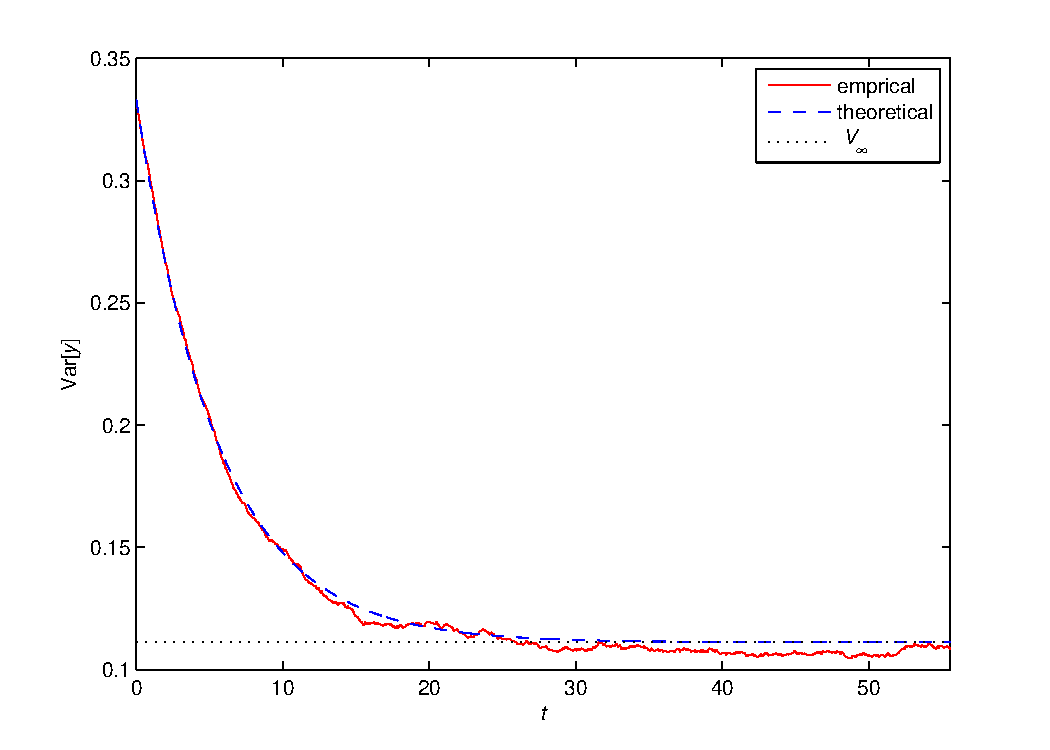
\includegraphics[width=0.8\textwidth]{./chapter_3/figs/var_wealth.pdf}
\caption{Wealth tax. The empirical variance of the rescaled wealths of $N=10^4$ realisations of 
\eref{wsde} with uniformly-distributed initial wealths (red); the theoretical variance for the infinite 
ensemble, $V(t)$ (blue dashed); and the asymptotic theoretical variance, $V_\infty$ (black dotted). 
Parameter values are $\mu=0.05$, $\sigma^2=0.02$, and $\tau=0.1$ per unit time.}
\flabel{var_wealth}
\ec
\end{figure}
\fref{hist_wealth} shows the initial distribution of rescaled wealths, which was chosen to be uniform, 
and the final distribution at the end of the period shown in \fref{var_wealth}.
\begin{figure}
\bc
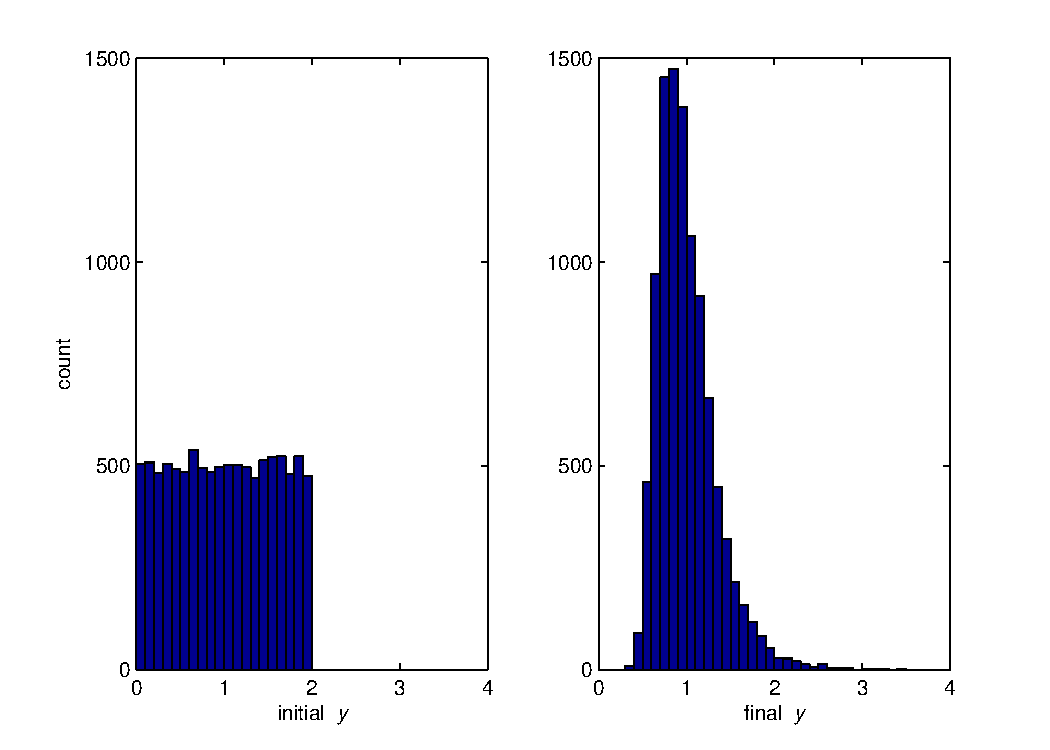
\includegraphics[width=0.8\textwidth]{./chapter_3/figs/hist_wealth.pdf}
\caption{Histograms of the initial (left) and final (right) empirical distributions of the rescaled 
wealth for the same realisations of \eref{wsde} used in \fref{var_wealth}.}
\flabel{hist_wealth}
\ec
\end{figure}

The simulated parameter values give a critical tax rate of 1\% pa. This is broadly in line 
with genuine annual wealth and property taxes in the few countries in which they are 
levied. Under the simulated tax rate of 10\% pa, the stabilisation time is $T_s\approx6$ 
years. It is hard to imagine a wealth tax of this magnitude being politically feasible in the 
real world. In our simple model, the tax rate could be set either to achieve convergence 
of inequality to a desired level, reflected by $V_\infty$, or over a desired timescale, 
represented by $T_s$.

It is interesting to connect this with the most widely levied wealth tax: the inheritance 
tax. In the UK this is levied at 40\% of the value of an individual's estate (above a 
certain threshold) upon death. We can surmise that an individual will typically hold 
most of his wealth for the human generation time of around 30 years, this being a 
sensible estimate of the time between inheriting or otherwise accumulating his wealth 
and passing it on. Using our plausible parameter values, an inheritance tax of 40\% 
corresonds to an annually compounded wealth tax of $1-(0.6)^{1/30} \approx 1.7\%$ 
pa and a stabilisation time of around 70 years. The former is close to and, notably, 
above the critical rate of 1\% pa, suggesting that variance stabilisation may be an 
influential criterion in the determination of our taxes.

\subsubsection{Income tax}
\seclabel{Income_tax}
In our very simple model, we have seen that a flat wealth tax can stabilize
the variance of the rescaled-wealth distribution. In this section we show 
that in a similarly simple model an income tax can achieve the same result. 
We introduce a model of income tax under which a fraction, $0\leq\tau\leq1$, of 
each individual's determinsitic wealth increment, $\mu x\,dt$, is deducted and 
the total tax raised is redistributed equally. This is modelled by the stochastic wealth process,
\be
dx = x[\mu(1-\tau)\,dt + \sigma\,dW] + \mu\tau\ave{x}_N dt.
\elabel{isde}
\ee
Again, we consider the large-population limit $N\to\infty$, corresponding to the replacement 
$\ave{x}_N\to\ave{x}$. For positive drift, $\mu>0$, the deterministic increment, $\mu x\,dt$, is guaranteed to 
be positive. It can be thought of as the income derived from that individual's activities, 
such as employment, on which governments typically levy taxes. Note that $\tau$ in \eref{isde} is a dimensionless number, whereas it is
a rate of dimension ``per unit time'' in \eref{wsde}. The form of 
\eref{isde} is identical to \eref{wsde} with the parameter transformation 
$\tau\rightarrow\mu\tau$. Thus we can immediately deduce the dynamic for the rescaled wealth as
\be
dy = y(-\mu\tau\,dt + \sigma\,dW) + \mu\tau\,dt.
\elabel{itax}
\ee
The variance stabilisation condition analogous to \eref{wstab} becomes
\be
\boxed{
\tau > \tau_c \equiv \frac{\sigma^2}{2\mu}.
}
\elabel{icrit}
\ee
This defines the critical income tax, $\tau_c$, above which the variance converges to its asymptotic value,
\be
V_\infty = \frac{\sigma^2}{2\mu\tau-\sigma^2},
\ee
according to
\be
V(t) = V_\infty + (V_0 - V_\infty) e^{-(2\mu\tau-\sigma^2)t}.
\elabel{ivar}
\ee
Finally, the stabilisation time is
\be
T_s = \frac{1}{2\mu\tau - \sigma^2}.
\ee

\fref{var_income} compares the evolution of the empirical variance of the rescaled wealths of $10^4$ realisations of the stochastic wealth process in \eref{isde} with the theoretical result for the infinite ensemble. Parameter values were $\mu=0.05$ and $\sigma^2=0.02$ per unit time, and $\tau=0.45$. The latter is the UK's limiting income tax rate for large incomes, which will be the determining tax rate for variance stabilisation.
\begin{figure}
\bc
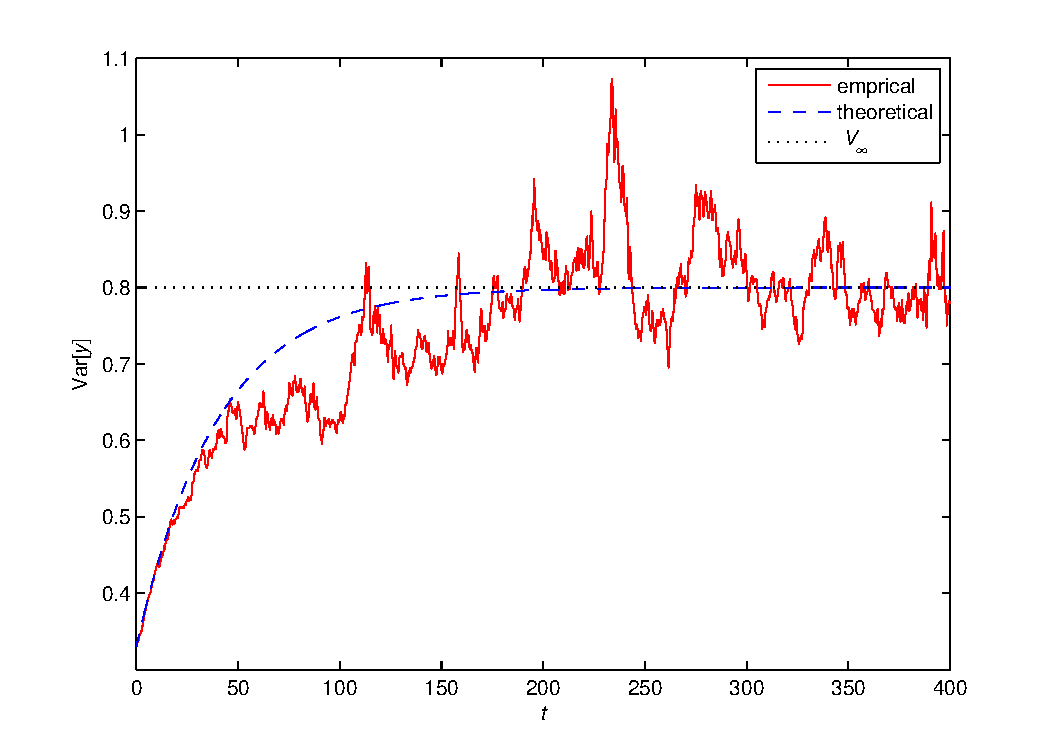
\includegraphics[width=0.8\textwidth]{./chapter_3/figs/var_income.pdf}
\caption{Income tax. The empirical variance of the rescaled wealths of $10^4$ realisations of \eref{isde} with uniformly-distributed initial wealths (red); the theoretical variance for the infinite ensemble, $V(t)$ (blue dashed); and the asymptotic theoretical variance, $V_\infty$ (black dotted). Parameter values are $\mu=0.05$ and $\sigma^2=0.02$ per unit time, and $\tau=0.45$.}
\flabel{var_income}
\ec
\end{figure}

The finite-sample deviations from the infinite-ensemble result are larger in \fref{var_income} 
than in \fref{var_wealth}. This is due entirely to the simulated parameter values: \eref{wsde} 
and \eref{isde} can be made equivalent by choosing different parameters. 
%Quantifying the scales of the finite-sample effects, and particularly their dependence 
%on $\tau$, would go some way towards illustrating the difference in the stabilisation 
%properties of the two taxation types under potentially realistic tax rates. This may be 
%a worthwile project.

\fref{hist_income} shows the initial distribution of rescaled wealths, which was chosen to be uniform, and the final distribution at the end of the period shown in \fref{var_income}.
\begin{figure}
\bc
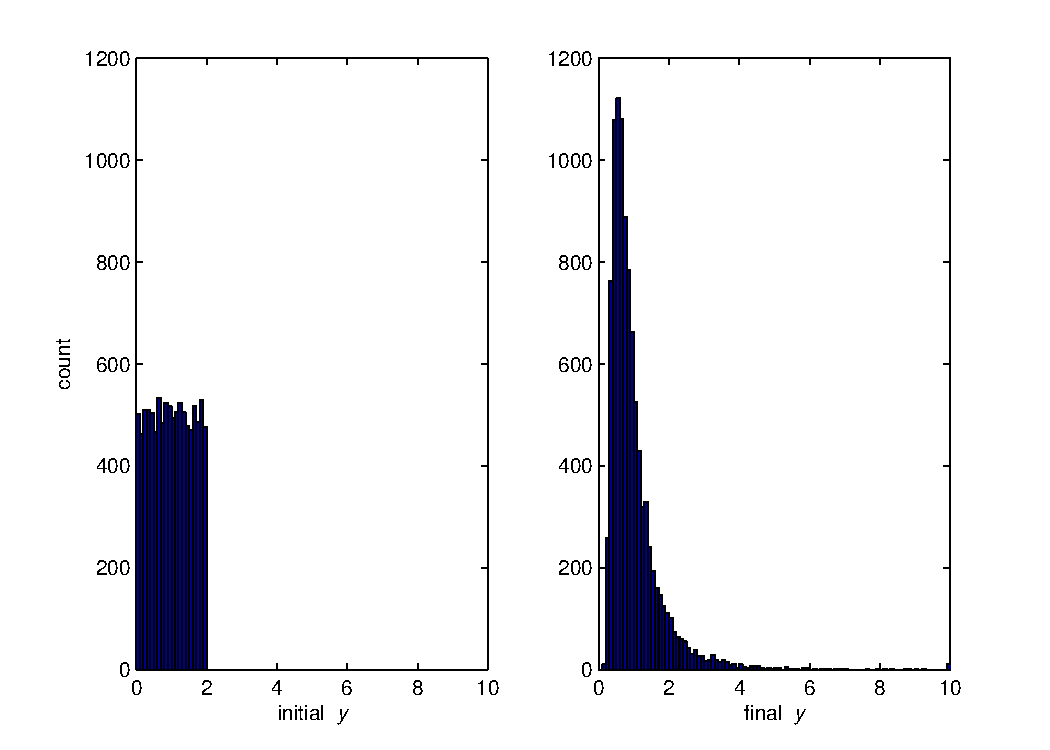
\includegraphics[width=0.8\textwidth]{./chapter_3/figs/hist_income.pdf}
\caption{Histograms of the initial (left) and final (right) empirical distributions of the rescaled wealth for the same realisations of \eref{itax} used in \fref{var_income}.}
\flabel{hist_income}
\ec
\end{figure}
The distribution of wealths under income tax has an appreciably longer tail than under wealth tax. As before this is a function of the parameter choices. The simulated parameter values have a critical income tax rate of $\tau_c=0.2$ and a stabilisation time of $T_s=40$ years. Thus the UK sets its income tax at a level which, at least in this simple framework, has a variance stabilising effect.
\FloatBarrier
%
%\bibliographystyle{abbrv}
%\bibliography{./../bibliography}
%
%\end{document}